\documentclass[11pt]{article} %taille de la police par défaut, et équations jusitifées à gauche
\usepackage[top=2.54cm,bottom=2.54cm,left=2.54cm,right=2.54cm,a4paper]{geometry}
\usepackage{xcolor}
\usepackage{hyperref}
\usepackage{url}
\usepackage[utf8]{inputenc} % lettres accentuées
\usepackage[T1]{fontenc}    % Use 8-bit encoding that has 256 glyphs
\usepackage[english]{babel} % Pour le français
\usepackage{graphicx}       % Pour inclure des images
\graphicspath{{images/}}    % Où sont les images ?

\usepackage{listings}      % Pour coloriser les codes que vous insérez
%\lstset{ %
%  backgroundcolor=\color{white},   % choose the background color; you must add \usepackage{color}
%  basicstyle=\footnotesize\ttfamily,        % the size of the fonts that are used for the code
%  breakatwhitespace=false,         % sets if automatic breaks should only happen at whitespace
%  breaklines=true,                 % sets automatic line breaking
%  captionpos=b,                    % sets the caption-position to bottom
%  commentstyle=\color{F18E00},    % comment style
%  deletekeywords={...},            % if you want to delete keywords from the given language
%  escapeinside={\%*}{*)},          % if you want to add LaTeX within your code
%  extendedchars=true,              % lets you use non-ASCII characters; for 8-bits encodings only, does not work with UTF-8
%  %frame=single,                    % adds a frame around the code
%  keepspaces=true,                 % keeps spaces in text, useful for keeping indentation of code (possibly needs columns=flexible)
%  %language=Octave,                 % the language of the code
%  morekeywords={*,...},            % if you want to add more keywords to the set
%  numbers=left,                    % where to put the line-numbers; possible values are (none, left, right)
%  numbersep=8pt,                   % how far the line-numbers are from the code
%  rulecolor=\color{black},         % if not set, the frame-color may be changed on line-breaks within not-black text (e.g. comments (green here))
%  showspaces=false,                % show spaces everywhere adding particular underscores; it overrides 'showstringspaces'
%  showstringspaces=false,          % underline spaces within strings only
%  showtabs=false,                  % show tabs within strings adding particular underscores
%  stepnumber=5,                    % the step between two line-numbers. If it's 1, each line will be numbered
%  tabsize=2,                       % sets default tabsize to 2 spaces
%}
%




\usepackage{booktabs}       % pour de jolis tableaux
%\usepackage{fancyhdr}       % pour des entêtes et pieds de pages améliorés.
\usepackage{hyperref}
\usepackage{makeidx}        % requis pour faire les index
\usepackage{amsmath}
\usepackage{amsfonts}
\usepackage{amssymb}
\usepackage{color}
\usepackage{array}
\usepackage{graphicx}
\usepackage{caption} 
\usepackage{hyperref}
\usepackage{algorithm}
\usepackage{algorithmic}
\usepackage{times}
\usepackage{enumitem}
\usepackage{tabularx}     % Ce fichier contient tous les packages nécessaires à la compilation

\title{ Cable Towing with an Autonomous Sailboat }
\author{Elouan Autret$^{1}$,Anna Friebe$^{2}$, Ronny Eriksson$^{3}$, Kjell Dahl$^{4}$, Matias Waller$^{5}$\\
\\
\normalsize{$^{1}$ ENSTA Bretagne, France, elouan.autret@ensta-bretagne.org}\\
\normalsize{$^{2}$ \r{A}land University, Finland, anna.friebe@ha.ax}\\
\normalsize{$^{3}$ \r{A}land University, Finland , ronny.eriksson@ha.ax}\\
\normalsize{$^{4}$ \r{A}land University, Finland, Kjell.Dahl@ha.ax}\\
\normalsize{$^{5}$ \r{A}land University, Finland, Matias.Waller@ha.ax}\\
}
\date{}

\begin{document}

\maketitle

\renewcommand{\contentsname}{Contents}	% Nom pour la table des matières
\renewcommand{\bibname}{Bibliography}	% Nom pour les références bibliographiques


\section*{Abstract}
Marine Research Platform \r{A}land Sailing Robots is a project at \r{A}land University of Applied  Sciences, with the goal to develop a mobile marine research platform using wind and solar energy. The platform will be evaluated for marine measurements and monitoring of harbor porpoise.

Monitoring of harbor porpoise, Phocoena phocoena, is often performed with Passive Acoustic Monitoring (PAM). To reach a sufficient depth to increase signaltonoise ratio hydrophnoes need to be towed on cable after the boat. The planned platform for towing a cable is a small autonomous sailboat at approximately 4 m length overall. This paper evaluates the possibility to tow a cable using such a platform.
   
Simulations of towing a cable have been performed. The dynamic model is described and evaluated. Test sailings with a boat similar to the planned platform towing a cable with a pressure sensor have been performed. Data from these tests are presented and compared to simulations. The ability of the model to capture the real behaviour is evaluated. The feasibility and limits of cable towing with a small autonomous sailboat are discussed.
   

%----------------------------------------------------------------------------------------
%	SOMMAIRE
%----------------------------------------------------------------------------------------
%\tableofcontents  % Imprime le sommaire
%\cleardoublepage  % pour commencer sur une page impaire

%%
%\listoffigures  % table des figures
%\listoftables   % table des tableaux
%%%----------------------------------------------------------------------------------------
%%%	PART I 
%%%----------------------------------------------------------------------------------------

\addcontentsline{toc}{chapter}{Introduction}
\section{Introduction}
The advances in making sailboat more autonomous open new perspective in a few domains, such as marine research, a boat that can stay at sea more than on day without surveillance and can change location where the user of the boat would want it to go. This is the goal of \r{A}land Sailing Robots a project of \r{A}land University of Applied Science (H\"{o}gskolan p\r{a} \r{A}land), developing a sailboat environment-friendly and usable in research, the project is funded by the European Regional Development Fund.

A research that the boat could do is the survey for harbour porpoises (\textit{Phocoena phocoen})in the Baltic sea as it an endangered species, in the current state there is fixed buoys to detect those animals in certain places,  but they does not cover every places, a autonomous sailboat would open the possibility of easy survey of any area not covered by the buoys without the noise created by a motorized manned boat.

\begin{figure}[H]
\centering
    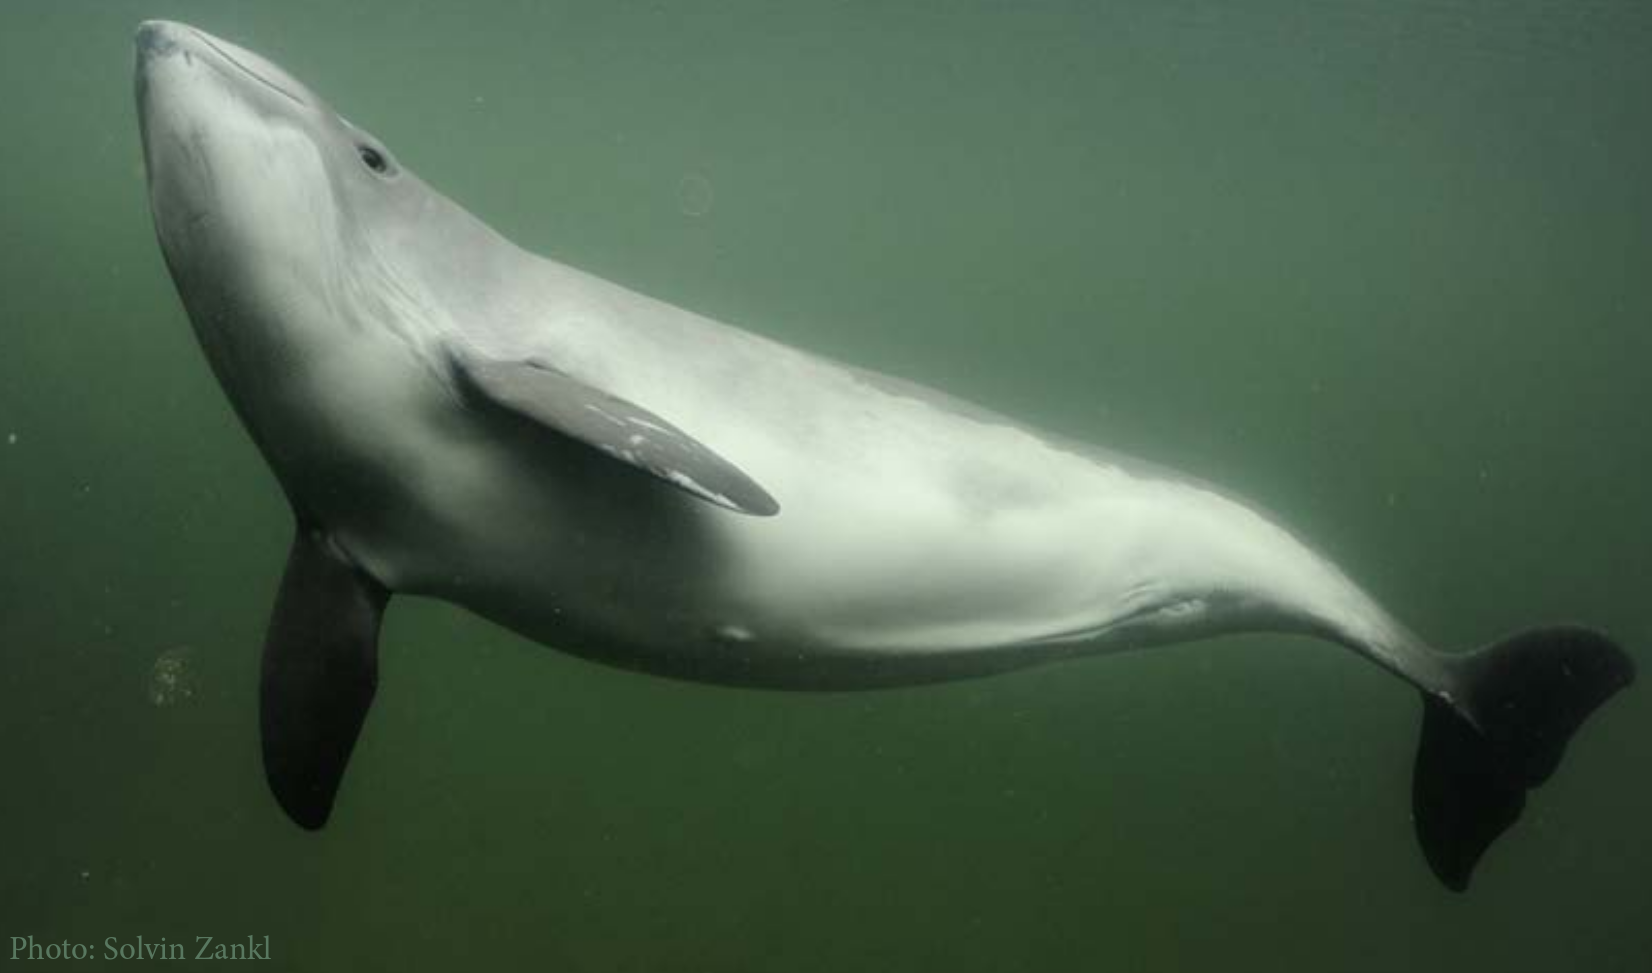
\includegraphics[scale=0.10,angle=0]{porpoise.png}
    \caption{Harbour Porpoise  photo: Solvin Zankl }
    \label{fig:porpoise}
\end{figure}

When using a boat the researcher need to have a cable, an array of hydrophones that will go deep enough to increase the signal-to-noise ratio because the surface of the sea create a lot of noise that would block the detection of the animals , a cable of hydrophones can reach 20 meters.


\begin{figure}[H]
\centering
    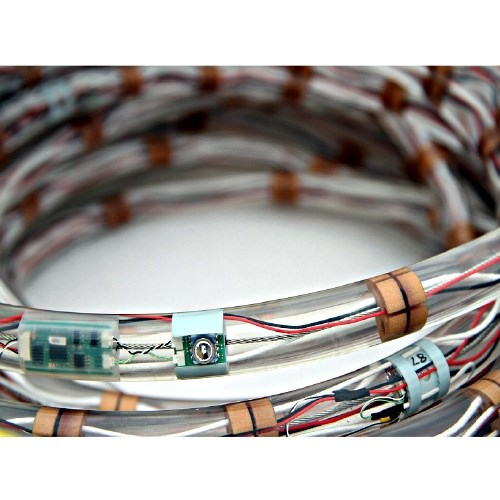
\includegraphics[scale=0.25,angle=0]{array_hydro.jpg}
    \caption{Array of Hydrophones NarcineArray from SEA }
    \label{fig:arrayHydro}
\end{figure}


The main goal of this report is to determine the viability of a small sailboat to carry such a cable. It will be done by simulation and field test. The modelling of a cable can be done with different ways such as finite elements for the more complicated solutions or by assimilating the cable as multiple connected rods. The last method as been chosen for the model. Following the work of~\cite{johansen2007modelling} (the goal was to not be dependent on a particular external software for multi-body dynamics).\\
The cable simulation will be then added to the modified sailboat model to take into account the effect of
the cable on the sailboat and model the behaviour of the boat and the cable.

Then tests have been done with the project sailboat, the result will be compared to the simulation and use to determine the possibilities of the towing sailboat.
%%
\section{Cable Simulation}
The choice of rods to model the cable was done because it seemed to be the simpler
way to get a good cable behaviour.

\section{SimMechanics\texttrademark ~Multi-Body Engine}

In order to get a model quickly, the use of an easy to made model was done with SimMechanics in Simulink.
The program allow to easily connect parts and their joints.The SimMechanics engine will be handling the movement of the cable and the effect of forces on it.

\begin{figure}[H]
\centering
    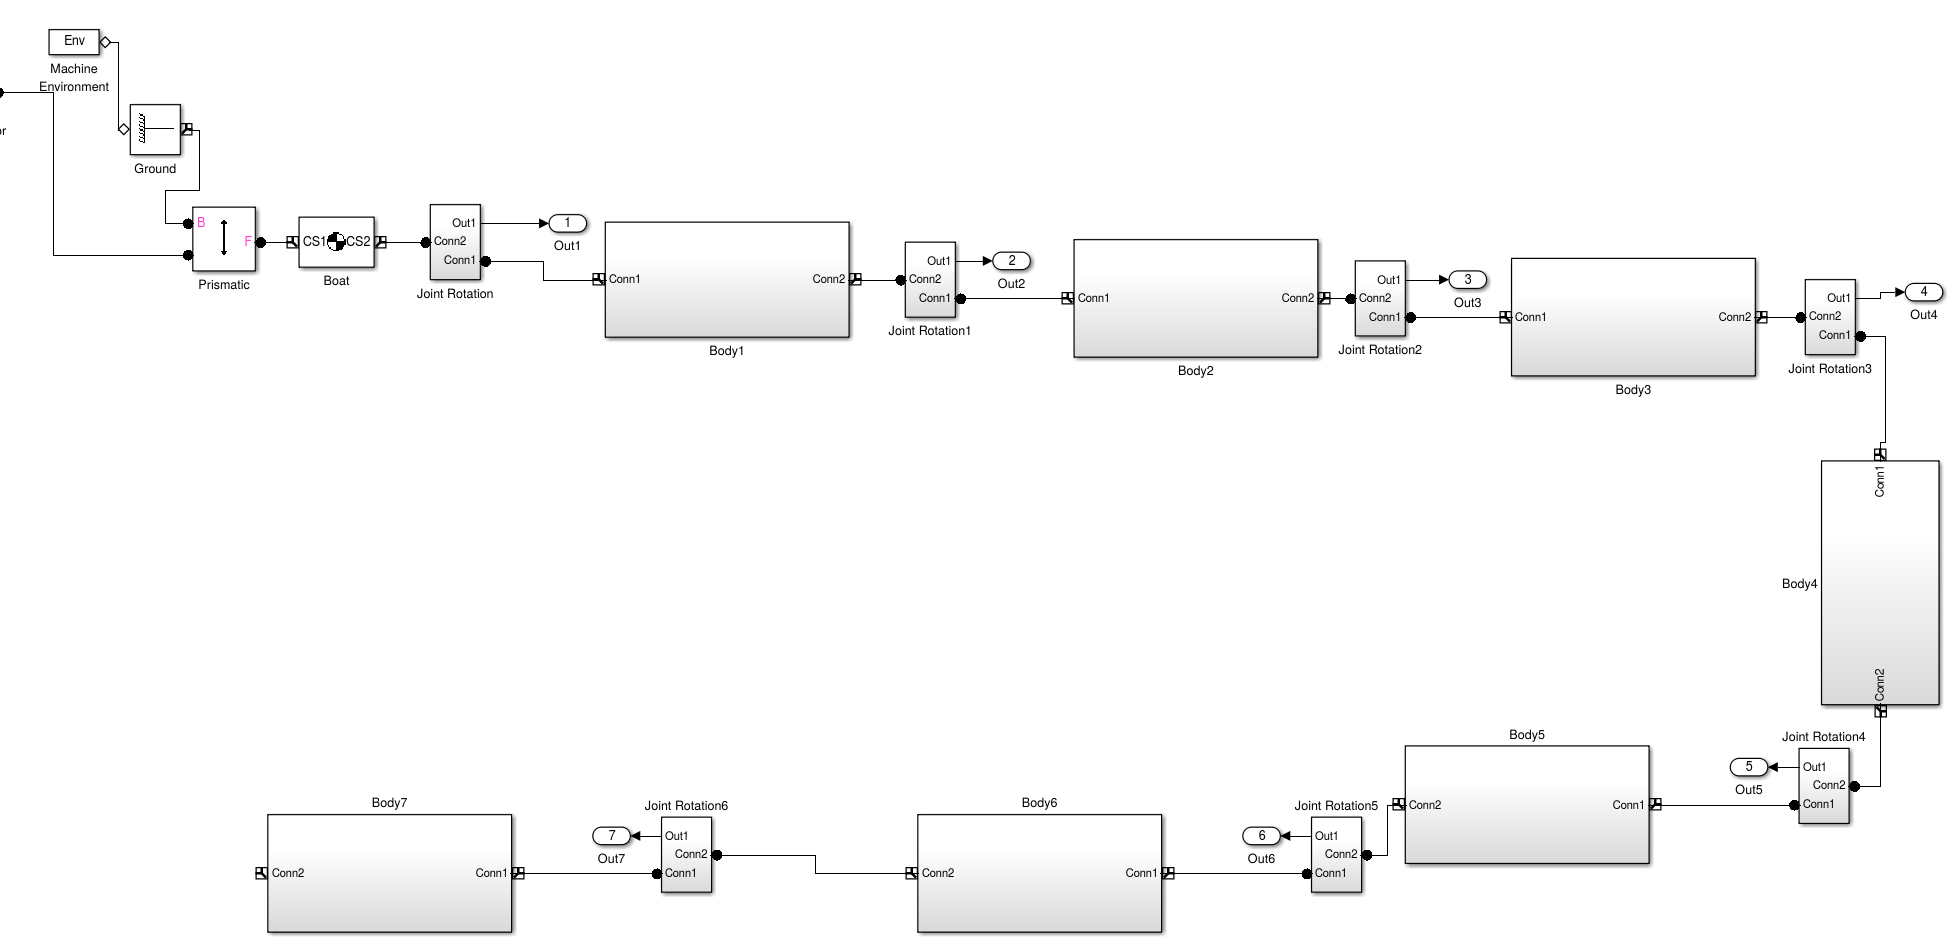
\includegraphics[scale=0.2,angle=0]{MultyBodySimMech.png}
    \caption{Simulink Model of the Cable.}
    \label{fig:SimulinkFullMod}
\end{figure}

The implementation of the model in Simulink is done in a graphic way (see~\ref{fig:SimulinkFullMod}). In
this first model the cable is modelled via seven rods connected via 2 degree of freedom joints, which are rotations.

\begin{figure}[H]
\centering
    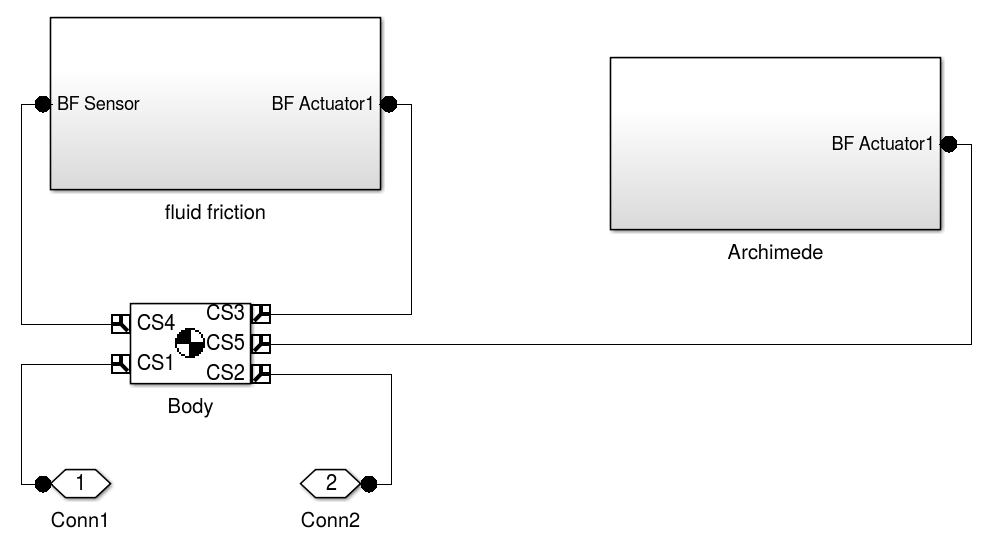
\includegraphics[scale=0.35,angle=0]{rod_pic.png}
    \caption{Single rod, a part of the cable.}
    \label{fig:SingleRod}
\end{figure}

Each rod is represented by a body, the object handled by SimMechanics, this body got a mass and an inertia matrix,here the inertia for a cylinder has been chosen. Then the application points of the forces and joints are
initialized.

The gravity is automatically computed by SimMechanics but not other optionals forces (at least for the first generation) such as the fluid friction and the Archimedes principle. 

\begin{figure}[H]
\centering
    \begin{minipage}[b]{0.4\textwidth}
    \centering
    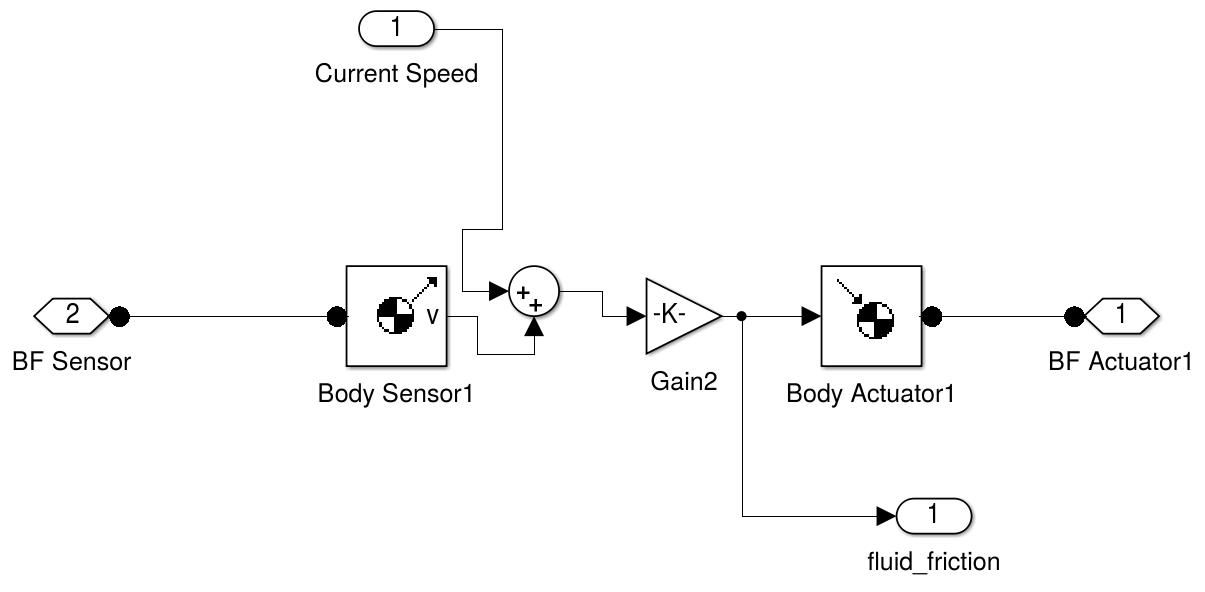
\includegraphics[scale=0.2,angle=0]{fluidfrictionSimMech.png}
    \caption{Computation of the fluid friction forces in Simulink.}
    \label{fig:fluidSimMech}
    \end{minipage}
    \hfill
    \begin{minipage}[b]{0.4\textwidth}
    \centering
    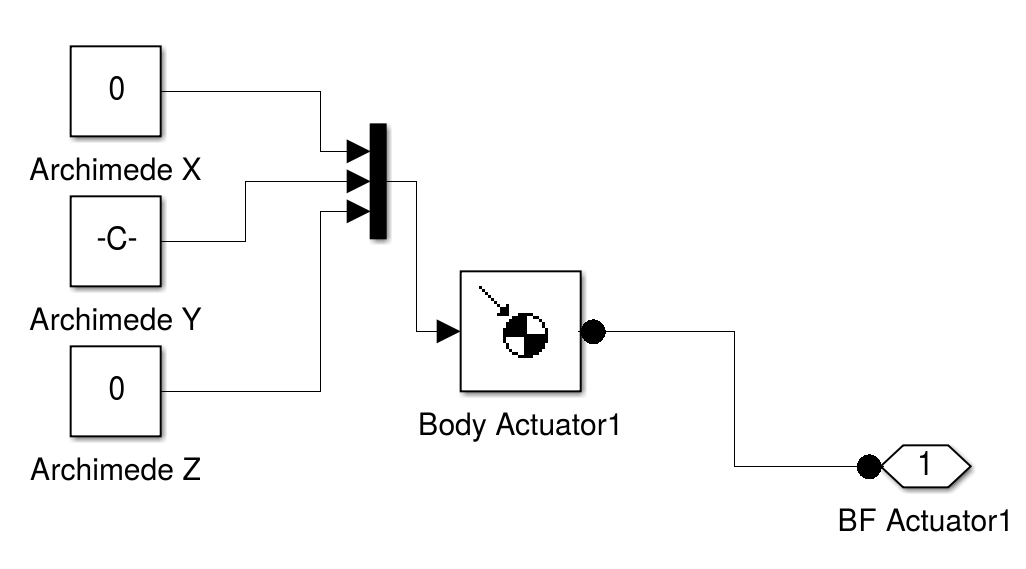
\includegraphics[scale=0.2,angle=0]{archiSimMech.png}
    \caption{Computation of the Archimedes force in Simulink.}
    \label{fig:archSimMech}
    \end{minipage}
\end{figure}

To compute the other forces SimMechanics allows the application of forces and torque on the body therefore, for each
body a sensor (see~\ref{fig:fluidSimMech}) output the velocity of the center of gravity of the rod, then the 
fluid friction is computed for each direction (the coefficient stay the same for each direction and pose of the cable in this model) to be applied on the body via an actuator \footnote{The video of the simulation can be see here \href{https://youtu.be/xEDApnU54ac}{Simulink video}.}.

\begin{figure}[H]
\centering
    \begin{minipage}[b]{0.5\textwidth}
    \centering
    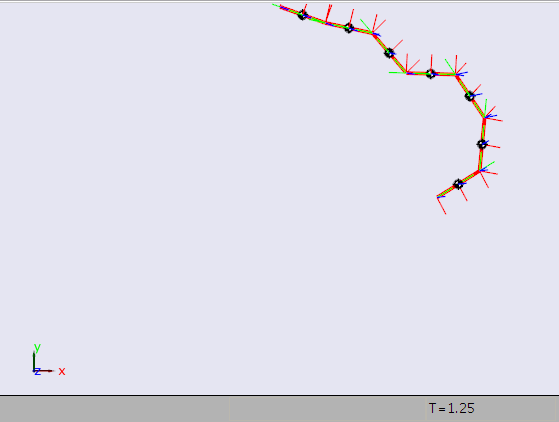
\includegraphics[scale=0.4,angle=0]{cable_simu2.png}
    \caption{Output of the Simulink simulation with random pose at the start.}
    \label{fig:Out1SimMech}
    \end{minipage}
    \hfill
    \begin{minipage}[b]{0.45\textwidth}
    \centering
    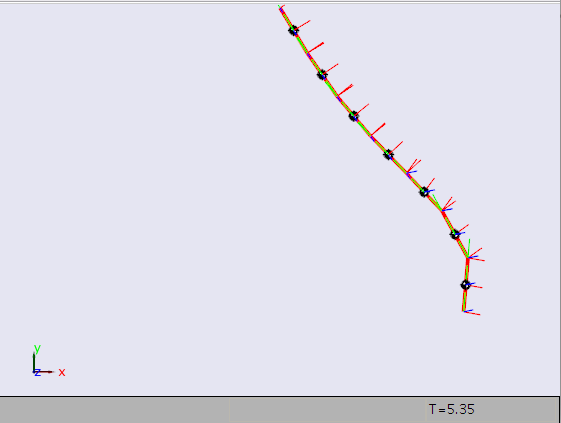
\includegraphics[scale=0.4,angle=0]{cable_simu1.png}
    \caption{Output of the Simulink simulation a few second later than~\ref{fig:Out1SimMech}.}
    \label{fig:Out2SimMech}
    \end{minipage}
\end{figure}


More simulation has been made to determine the behaviour of the cable, mainly the cable is attached on a point following a strict line with a constant speed, the cable is towed but has no action on the towing point for the moment.

\begin{figure}[H]
\centering
    \begin{minipage}[b]{0.4\textwidth}
    \centering
    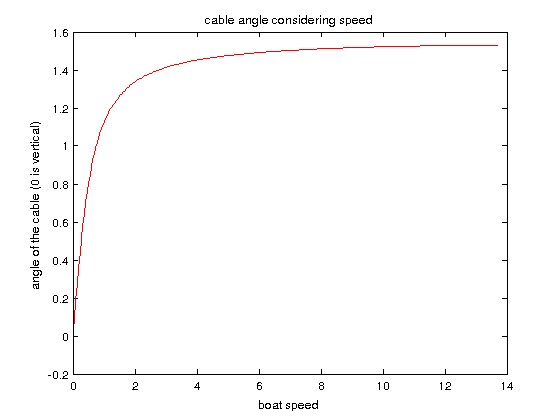
\includegraphics[scale=0.45,angle=0]{angle_over_speed_r.png}
    \caption{Angle of the cable to the vertical depending on the speed of the boat.}
    \label{fig:angleSpeed}
    \end{minipage}
    \hfill
    \begin{minipage}[b]{0.45\textwidth}
    \centering
    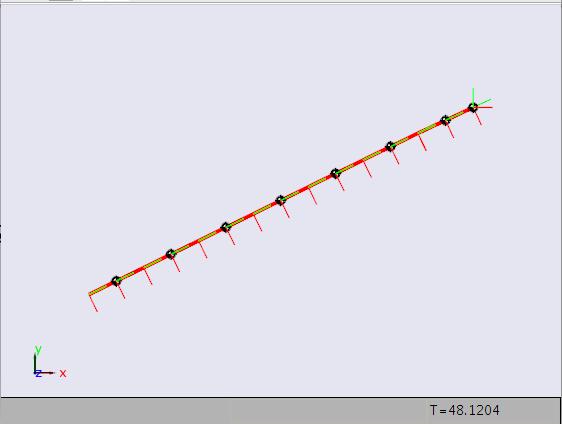
\includegraphics[scale=0.35,angle=0]{stabilized_cable.png}
    \caption{Output of a stabilized cable when towed by a particle with a constant and rectilinear motion.}
    \label{fig:stabCable}
    \end{minipage}
\end{figure}

In figure~\ref{fig:angleSpeed} is represented the angle of the cable to the vertical depending of the speed of the 
boat when the system is stabilized. The curve resemble to an inverse curve dependant on the density of the cable.
It means beyond a certain velocity the cable will be useless due to be not enough submerged.

\begin{figure}[H]
\centering
    \begin{minipage}[b]{0.4\textwidth}
    \centering
    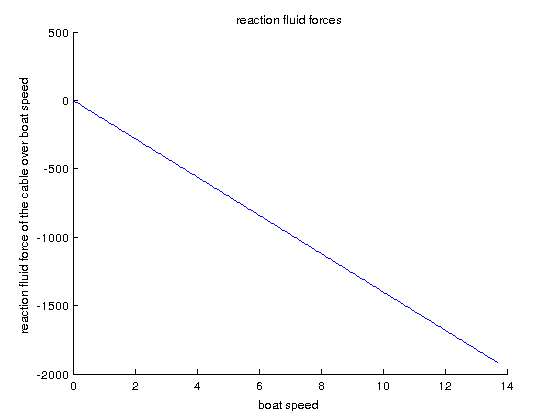
\includegraphics[scale=0.45,angle=0]{fluid_forces_over_speed.png}
    \caption{Resultant of the fluid forces when stabilized depending on the speed.}
    \label{fig:fluidSpeed}
    \end{minipage}
    \hfill
    \begin{minipage}[b]{0.45\textwidth}
    \centering
    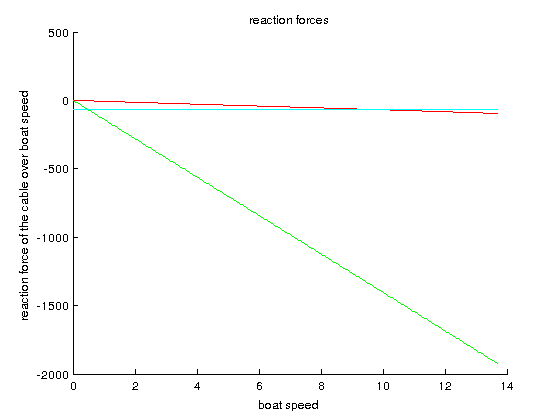
\includegraphics[scale=0.45,angle=0]{forces_over_speed_r.png}
    \caption{Resultant of forces on the joint boat-cable depending on the speed.}
    \label{fig:forceSpeed}
    \end{minipage}
\end{figure}

The result of the fluid friction forces (~\ref{fig:fluidSpeed}) is what was expected as the model use a linear friction which then can be extract from the the resultant at the junction point on the boat (~\ref{fig:forceSpeed} , cyan is horizontal force and green vertical force). Stabilized the force of the boat on the cable is equal to the force of the fluid on the cable which is logical as they are the only interaction on the horizontal axis (see \eqref{equ_Stab} where $\vec{P}$ is the gravitational force and $\vec{\Pi}$ represent the Archimedes principle).

%\begin{align}
\begin{equation}
 \vec{0} = \vec{f}_{cable/boat}+\vec{f}_{fluide}+\vec{P}+\vec{\Pi}\\
 \label{equ_Stab}
\end{equation}
%0 &= f_{cable/boat,x} + f_{fluide,x}\\
%0 &= f_{cable/boat,z} +f_{fluide,z}(0) + P_z+\Pi_z
%\end{align}

The same can be said on the vertical point with the sums of gravity and Archimedes principle equals the effects of the boat on the cable with no dependence with the speed.\\

The use of Simulink is easy and efficient but not everyone has the toolbox to use this simulation, so a more 
environment-free simulation is required.
\section{Independent cable Model}

This independent cable model is fully taken from  Vegar Johansen PhD thesis~\cite{johansen2007modelling} where the author present different to model a cable including the rod model. In this model the rods are modelled by vectors and centres of gravity.

A rod can characterised by the two following object:

\begin{align}
r &= \begin{bmatrix}
    r_x \\
    r_y \\
    r_z
\end{bmatrix}\, \textnormal{is the center of gravity}\\
b &= \begin{bmatrix}
    b_x \\
    b_y \\
    b_z
\end{bmatrix}\, \textnormal{is the vector for the rod orientation}
\end{align}

The forces acting on the cable are applied on the ends of each rods, meaning for example, the gravity force would be split in two forces acting on each side of the bar. Leading to the base formulas where a and b are the extremity of the bar:

\begin{align}
\ddot{r} &= \dfrac{1}{m}  (f_a+f_b) \\
\ddot{b} &=  \dfrac{6}{m}(f_a+f_b) - \dfrac{b}{L^{2}}  (\dfrac{6}{m}b^{T}(f_a+f_b)+\dot{b}^{T}\dot{b}) 
\end{align}

Then the model adds the use of the Baumgarte stabilization constraint~\cite{baumgarte1972stabilization} to respect the physical constraint on the bar , length and position of fixed points if there is, thus changing the precedent equation. 
The stabilization technique is a PID method therefore it depends on coefficient parameters, in a variable-step solver augmenting the P an D coefficient improve the simulation but will increase the time needed to do the simulation.

Johansen proposes three scenarios for this model, a free cable, a fixed-free scenario where one side of the cable is attached to a point and the last one is a fixed-fixed where both side are attached to points.
The model interesting for the modelling of the sailboat towing a cable is the fixed-free scenario where the attachment point is the boat.

\begin{figure}[H]
\centering
    \begin{minipage}[b]{0.4\textwidth}
    \centering
    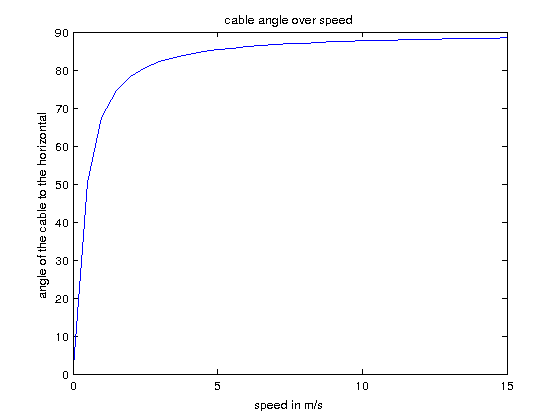
\includegraphics[scale=0.45,angle=0]{inde_cable_angle_speed.png}
    \caption{Angle of the cable when stabilized at the final speed.}
    \label{fig:angleIndSpeed}
    \end{minipage}
    \hfill
    \begin{minipage}[b]{0.45\textwidth}
    \centering
    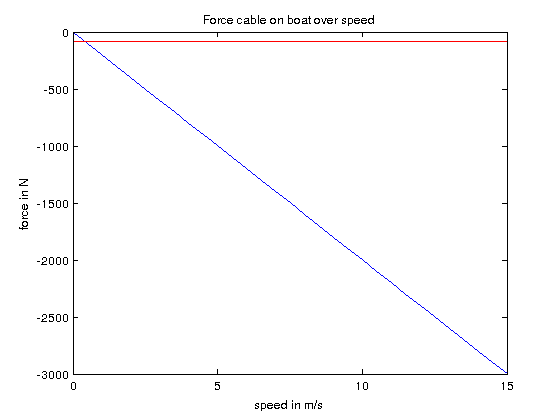
\includegraphics[scale=0.45,angle=0]{inde_cable_force_speed.png}
    \caption{Force of the cable on the boat when stabilized at the final speed.}
    \label{fig:forceIndSpeed}
    \end{minipage}
\end{figure}

By doing simulation with this model, the profile of the angle of the cable over speed is the same as in the Simulink model and the same can be done for the reaction of the cable on the boat, an constant for the vertical reaction and a linear decrease for the horizontal reaction dependant on the fluid friction force.

This model include a tolerance to errors which are resolved by the Baumgarte stabilisation technique but 
there still some left over:


\begin{figure}[H]
\centering
    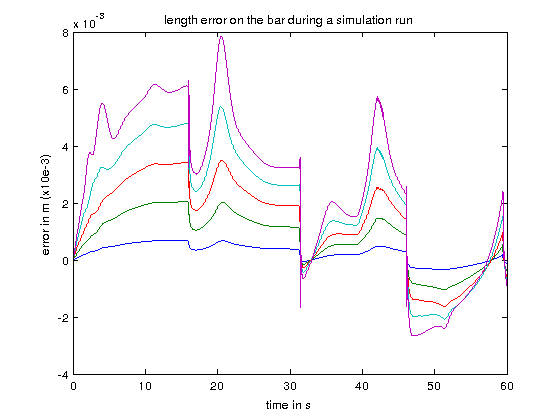
\includegraphics[scale=0.5,angle=0]{error_length_run.png}
    \caption{Error in length of the rods during a simulation run.}
    \label{fig:errorLRod}
\end{figure}

In the figure~\ref{fig:errorLRod} the error in length reach a maximum around one centimetre for a rod length of four meters\footnote{To see simulations : \href{https://www.youtube.com/watch?v=T7DRGq3E5x8}{Fixed cable video} or \href{https://www.youtube.com/watch?v=V4X0PsgsXZY to see simulations}{Moving cable with a constant speed video}}, this error can be considered negligible in this case but in some runs if the start is too sharp then, the simulation may diverge.

In this model each rod can have a different length and mass:

\begin{figure}[H]
\centering
    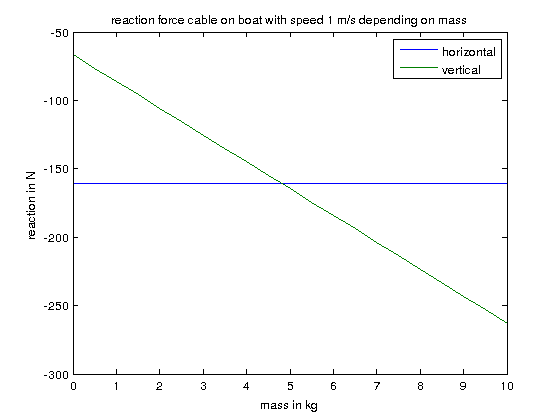
\includegraphics[scale=0.5,angle=0]{inde_cable_force_mass.png}
    \caption{Variation of reaction force of cable on boat depending on mass of last rod.}
    \label{fig:massForce}
\end{figure}

In figure~\ref{fig:massForce} is represented the force of the cable on the boat once stabilized and depending of the mass of the last rod. The horizontal force is constant over mass, this is logical as when stabilized mass does not appear in the horizontal part of the equation \eqref{equ_Stab}. And as for the vertical reaction it vary linearly with the mass,thus corresponding to the precedent equation on the z axis.

Changing the linear mass or the mass of the last rod have different effect on the final angle of the cable(see~\ref{fig:linmassAngle}).

\begin{figure}[H]
\centering
    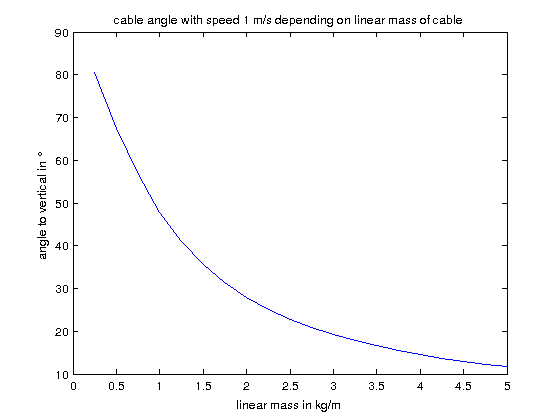
\includegraphics[scale=0.6,angle=0]{inde_cable_angle_linmass.png}
    \caption{Variation of the angle of the cable depending on the linear mass of the rods.}
    \label{fig:linmassAngle}
\end{figure}

To simulate this model there is more than one options, but to not make it diverge tweaking must be made.
If using a fixed-step size integration (Runge-Kutta,ODE45) the step need to be $\sim\mathcal{O}(10^{-3})$, it is the limit of this method and if the cable endure big acceleration it will diverge.

With an solver with variable step-size (ODE23) the result will be in general more accurate but the computation time became very high needing more than one second to compute one second of simulation.If possible Matlab coder should be used to help improve the computation time.


\section{Linking with Sailboat Simulation}
\section{Original Model}

The model of the sailboat come from~\cite{Melin2016} a modified version of the model in~\cite{LeBars2013}.


\begin{figure}[H]
\centering
    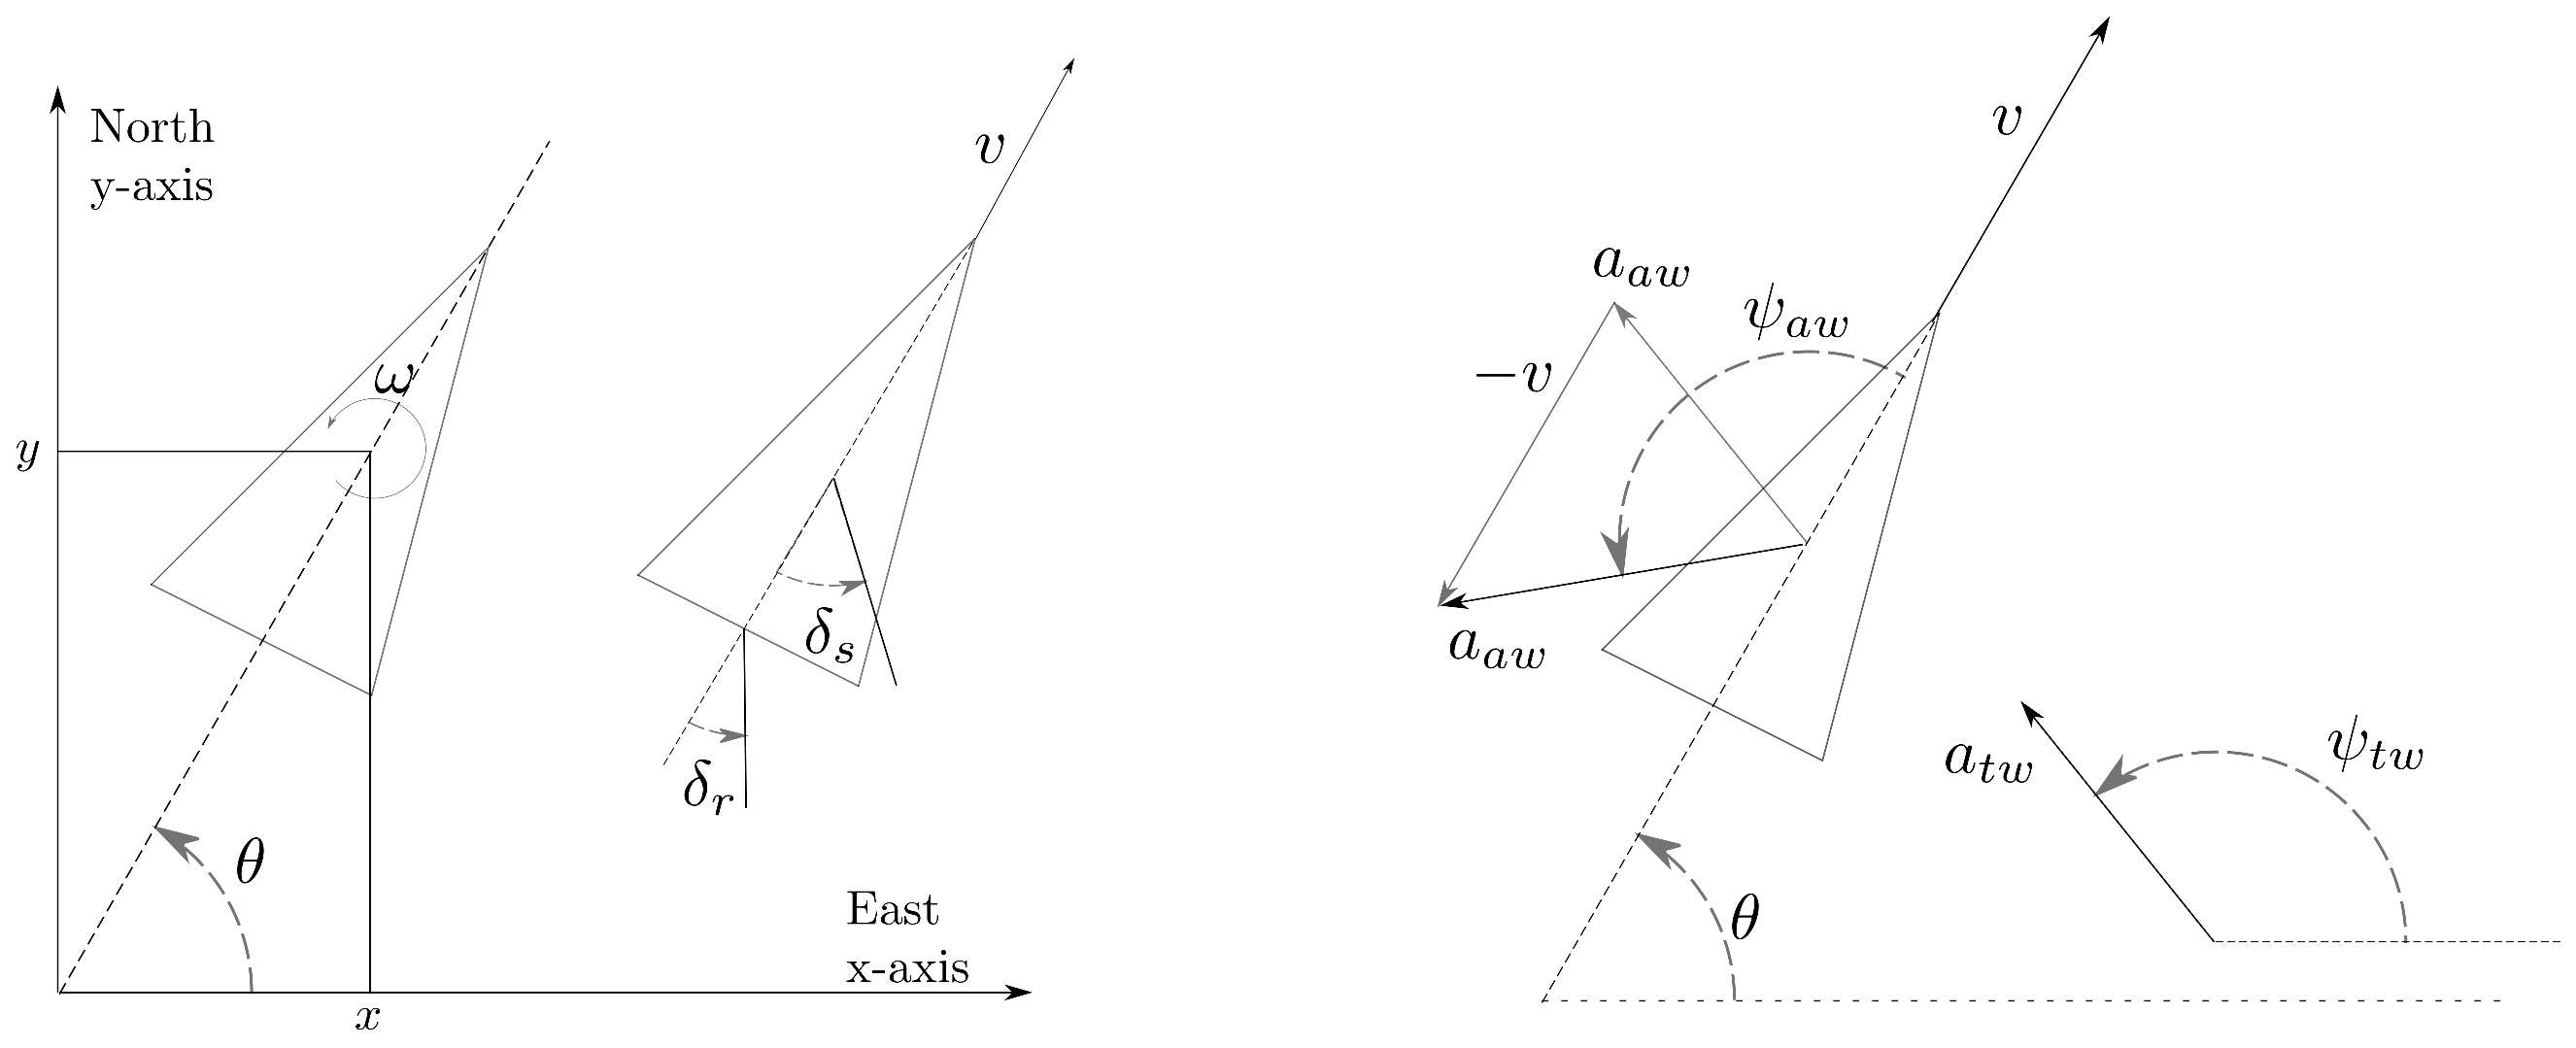
\includegraphics[scale=0.3,angle=0]{drawing_boat}
    \caption{Representation of the state vector variable and the inputs $\delta_s$ and $\delta_r$ and representation of the true wind and apparent wind.}
    \label{fig:drawing_boat_ink}
\end{figure}



\begin{equation}
\begin{bmatrix}
\dot{x}\\
\dot{y}\\
\dot{\theta}\\
\dot{v}\\
\dot{\omega}
\end{bmatrix}\  = \begin{bmatrix}
v \cos(\theta)+p_1 a_{tw} \cos(\psi_{tw})\\
v \sin(\theta)+p_1 a_{tw} \sin(\psi_{tw})\\
\omega\\
(g_s \sin(\delta_s)-g_r p_{11} \sin(\delta_r) - p_2 v^2)/p_9\\
(g_s(p_6-p_7\cos(\delta_s))-g_r p_8 \cos(\delta_r)-p_3 \omega v)/p_{10}
\end{bmatrix}
\end{equation}


The states boat is represented by different variables $x$ and $y$ for the position of the boat, a heading $\theta$ 
and an angular speed $\omega$.
The model is non-holonomic such as the boat will always go in the direction $\theta$ (minus the wind drift) therefore the speed $v$ is defined in the boat frame as for the input $[ \delta_s , \delta_r]$, where $\delta_r$ is the rudder angle and $\delta_s$ is the angle of the sail (which is proportional to the sheet length).


$g_s$ and $g_r$ are the force on the sail and on the rudder:
\begin{align}
g_s &= p_4 a_{aw} \sin(\delta_s - \psi_{aw})\\
g_r &= p_5 v^2 \sin(\delta_r)
\end{align}

The force on the sail depend on the apparent wind:

\begin{equation}
\bf{W}_{c,aw}= \begin{bmatrix}
a_{tw} \cos(\psi_{tw} -\theta) - v\\
a_{tw} \sin(\psi_{tw} -\theta)
\end{bmatrix}\
\end{equation}

\begin{equation}
\bf{W}_{p,aw}=\begin{bmatrix}
a_{aw}\\
\psi_{aw}
\end{bmatrix} = \begin{bmatrix}
\mid \bf{W}_{c,aw}\mid\\
\textnormal{angle}( \bf{W}_{c,aw})
\end{bmatrix}\
\end{equation}

$a_{tw}$ is the true wind speed and $\psi_{tw}$ its direction in the world frame
and $a_{aw}$ is the apparent wind speed on the boat and $\psi_{aw}$ the direction of the apparent wind in the boat frame.\\
\begin{minipage}{\linewidth}
\centering
\captionof{table}{Parameters correspondance} \label{tab:title2} 
\begin{center}
\begin{tabular}[t]{|c|l|l|}%{|m{0.10\linewidth}|m{0.3\linewidth}|m{0.1\linewidth}|}
\hline
 $p_1$ & drift coefficient & - \\ \hline
 $p_2$ & tangential friction & $kgs^{-1}$\\ \hline
 $p_3$ & angular friction & $kgm$ \\ \hline
 $p_4$ & sail lift & $kgs^{-1}$ \\ \hline
 $p_5$ & rudder lift & $kgs^{-1}$ \\ \hline
 $p_6$ & distance to sail & $m$ \\ \hline
 \end{tabular}
 \begin{tabular}[t]{|c|l|l|}%{|m{0.10\linewidth}|m{0.3\linewidth}|m{0.1\linewidth}|}
\hline
 $p_7$ & distance to mast & $m$ \\ \hline
 $p_8$ & distance to rudder & $m$ \\ \hline
 $p_9$ & mass of boat & $kg$ \\ \hline
 $p_{10}$ & moment of inertia & $kgm^2$ \\ \hline
 $p_{11}$ & rudder break coefficient & - \\ \hline
\end{tabular}
\end{center}
\end{minipage}
\bigskip

The goal of this model is to be simple, not to experience the real reaction of a sailboat but
to be able to implement a controller for this ship. This kind of reasoning has been successful in the past 
with this model and others (see~\cite{LeBars2013}~\cite{Melin2016}).

\section{Adding the cable force}

The design of this model originated from the model in this paper~\cite{Jaulin2015} and changed after that.
This model will separate the cable simulation and the sailboat. Having a cable on the boat, changes its dynamic 
and the model need to be updated to take into account the new forces applying on the boat.
\subsection{Modification of this model}
\paragraph*{Adding drifting}
~\\
%\vskip1mm
\hskip7mm 

Having a cable on the boat will make it not follow the normal path 
Here $\alpha_{c}$ is the direction of the force of the cable on the boat in the world frame and $g_c$ its norm.
$v_c$ represent the effect of the cable on the boat, it doesn't depend on the direction of boat when calculating its speed, and $\alpha_{v}$ is the direction of this drift. 


\begin{equation}
\begin{bmatrix}
\dot{x}\\
\dot{y}\\
\dot{\theta}\\
\dot{v}\\
\dot{v_{c,x}}\\
\dot{v_{c,y}}\\
\dot{\omega}
\end{bmatrix}\  = \begin{bmatrix}
v \cos(\theta)+v_{c,x}+p_1 a_{tw} \cos(\psi_{tw})\\
v \sin(\theta)+v_{c,y}+p_1 a_{tw} \sin(\psi_{tw})\\
\omega\\
(g_s \sin(\delta_s)-g_r p_{11} \sin(\delta_r)+ g_c \cos(\alpha_c-\theta) - p_2 v^2)/p_9\\
(-(p_2+p_{12} \sin^2(\alpha_v-\theta))(v_{c,x} \mid v_{c,x} \mid ) + g_c \sin(\alpha_{c} -\theta) \cos(\theta+\pi/2))/p_9\\
(-(p_2+p_{12} \sin^2(\alpha_v-\theta))(v_{c,y} \mid v_{c,y} \mid ) + g_c \sin(\alpha_{c} -\theta) \sin(\theta+\pi/2))/p_9\\
(g_s(p_6-p_7\cos(\delta_s))-g_r p_8 \cos(\delta_r)-p_3 \omega v)/p_{10}
\end{bmatrix}
\end{equation}

But the effect this drifting depend on the direction of the boat.
If the drift make the boat go in a orthogonal direction the friction of the boat will be more important than if it
drag the boat on the same direction therefore the computation of friction :

\begin{equation}
\textnormal{friction} = (p_2+p_{12} \sin^2(\alpha_v-\theta))
\end{equation}

When $\alpha_v = \theta \pmod{\pi}$ the boat goes in the same direction of the drift therefore the friction is equal to the tangential friction $p_2$. But when $\alpha_v -\theta =\pm \pi/2$ the friction created by the drift is orthogonal to the boat so the friction is at its maximum.

But the cable does not always make the boat drift, if the cable pull in the same direction of the boat, the force 
will directly impact the speed  $v$ of the boat (without making it drift). The effect of the cable is distributed between $\dot{v}$ and $\dot{v_c}$ depending on the difference $\alpha_c -\theta$.

\paragraph*{Changing Application point of the force from the cable}
~\\
\vskip1mm
\hskip7mm
 
The point of effect of the cable force may not be at the center of inertia of the boat therefore it will
have an effect on the angular acceleration. The angular acceleration formula is changed to the following  when
the cable is place on the median of the boat:
\begin{equation}
\dot{\omega} =
(g_s(p_6-p_7\cos(\delta_s))-g_r p_8 \cos(\delta_r)-p_3 \omega v -p_{13} g_c \sin(\alpha_c-\theta))/p_{10}
\end{equation}

With $-p_{13} g_c \sin(\alpha_c-\theta)$ being the effect of the cable on the angular acceleration.
This mean the cable will often have a breaking effect to the rotation of the boat.

\begin{figure}[H]
\centering
    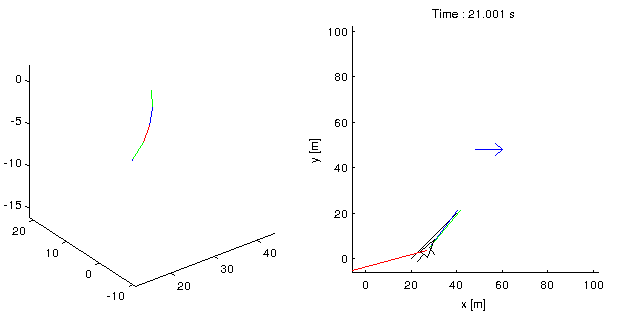
\includegraphics[scale=0.7,angle=0]{under_way_cable_no_delay.png}
    \caption{Simulation display representing first the cable, then the boat.}
    \label{fig:3wayBoat}
\end{figure}

In figure~\ref{fig:3wayBoat} is represented the cable \footnote{To see simulation : \href{https://www.youtube.com/watch?v=1nrbdikXr8A}{Simulation of a boat with a cable on it}},and the boat with in red the force of the cable on the boat and the blue arrow is the wind direction.

\subsection{Simulation Results}

The boat behave differently whereas it have a cable attached or not. The boat is slower and have a longer response time also.

\begin{figure}[H]
\centering
    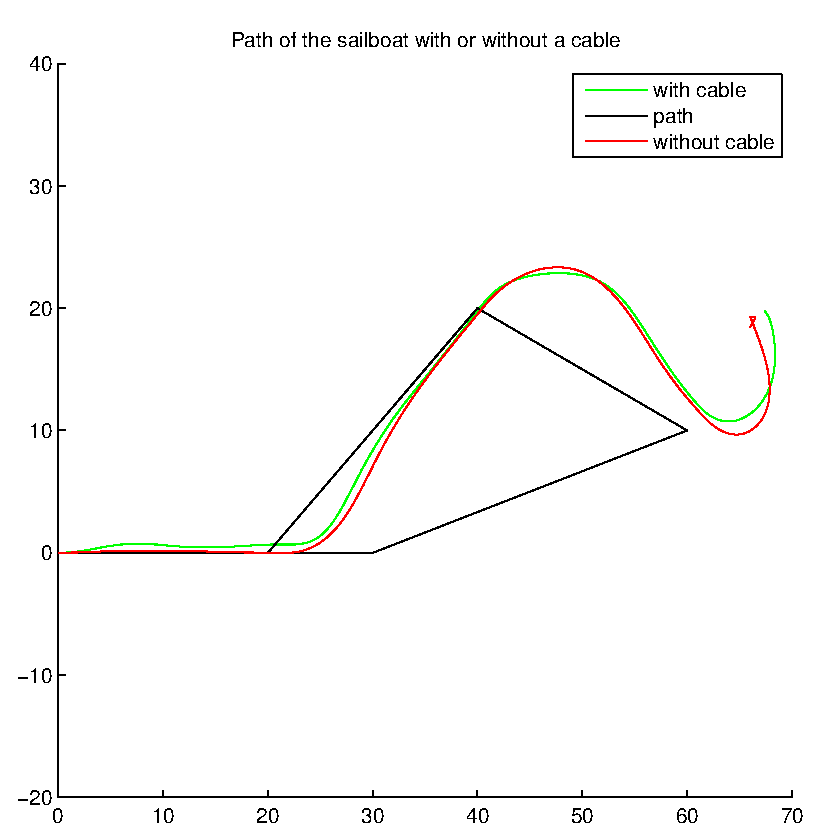
\includegraphics[scale=0.4,angle=0]{path_w_wtFig}
    \caption{Path taken by the boat with or without cable.}
    \label{fig:pathBoat}
\end{figure}

In figure~\ref{fig:pathBoat} the path of the boat with or without cable is represented, the boat is controlled each time by the algorithm from Le Bars and Jaulin 2013~\cite{LeBars2013}. The boat is less controllable in a straight
line, indeed the boat start at the position zero in the direction of the wind, the boat without cable follow very thoroughly the line but the boat with cable discard from the line.

The boat with cable looks more efficient when turning, but it would be because of the lesser speed.



\section{Viability of the model}
To test the model, a cable with a pressure sensor has been put on the boat in order to capture the behaviour of the cable.



\section*{Boat specification}

The boat is a retrofitted version of the model Mini-12 and can be consider of the 2.4mR-class by the International Sailing Federation meaning is length is around 4 meters. It weigh around 300 kg.

To proceed to the measurement of the cable depth, a pressure sensor has been added and also an Arduino  Uno as  Analog to digital converter and send the sensor data to the computing unit a Raspberry Pi 3 Model B.

\begin{figure}[H]
\centering
    \begin{minipage}[b]{0.4\textwidth}
    \centering
    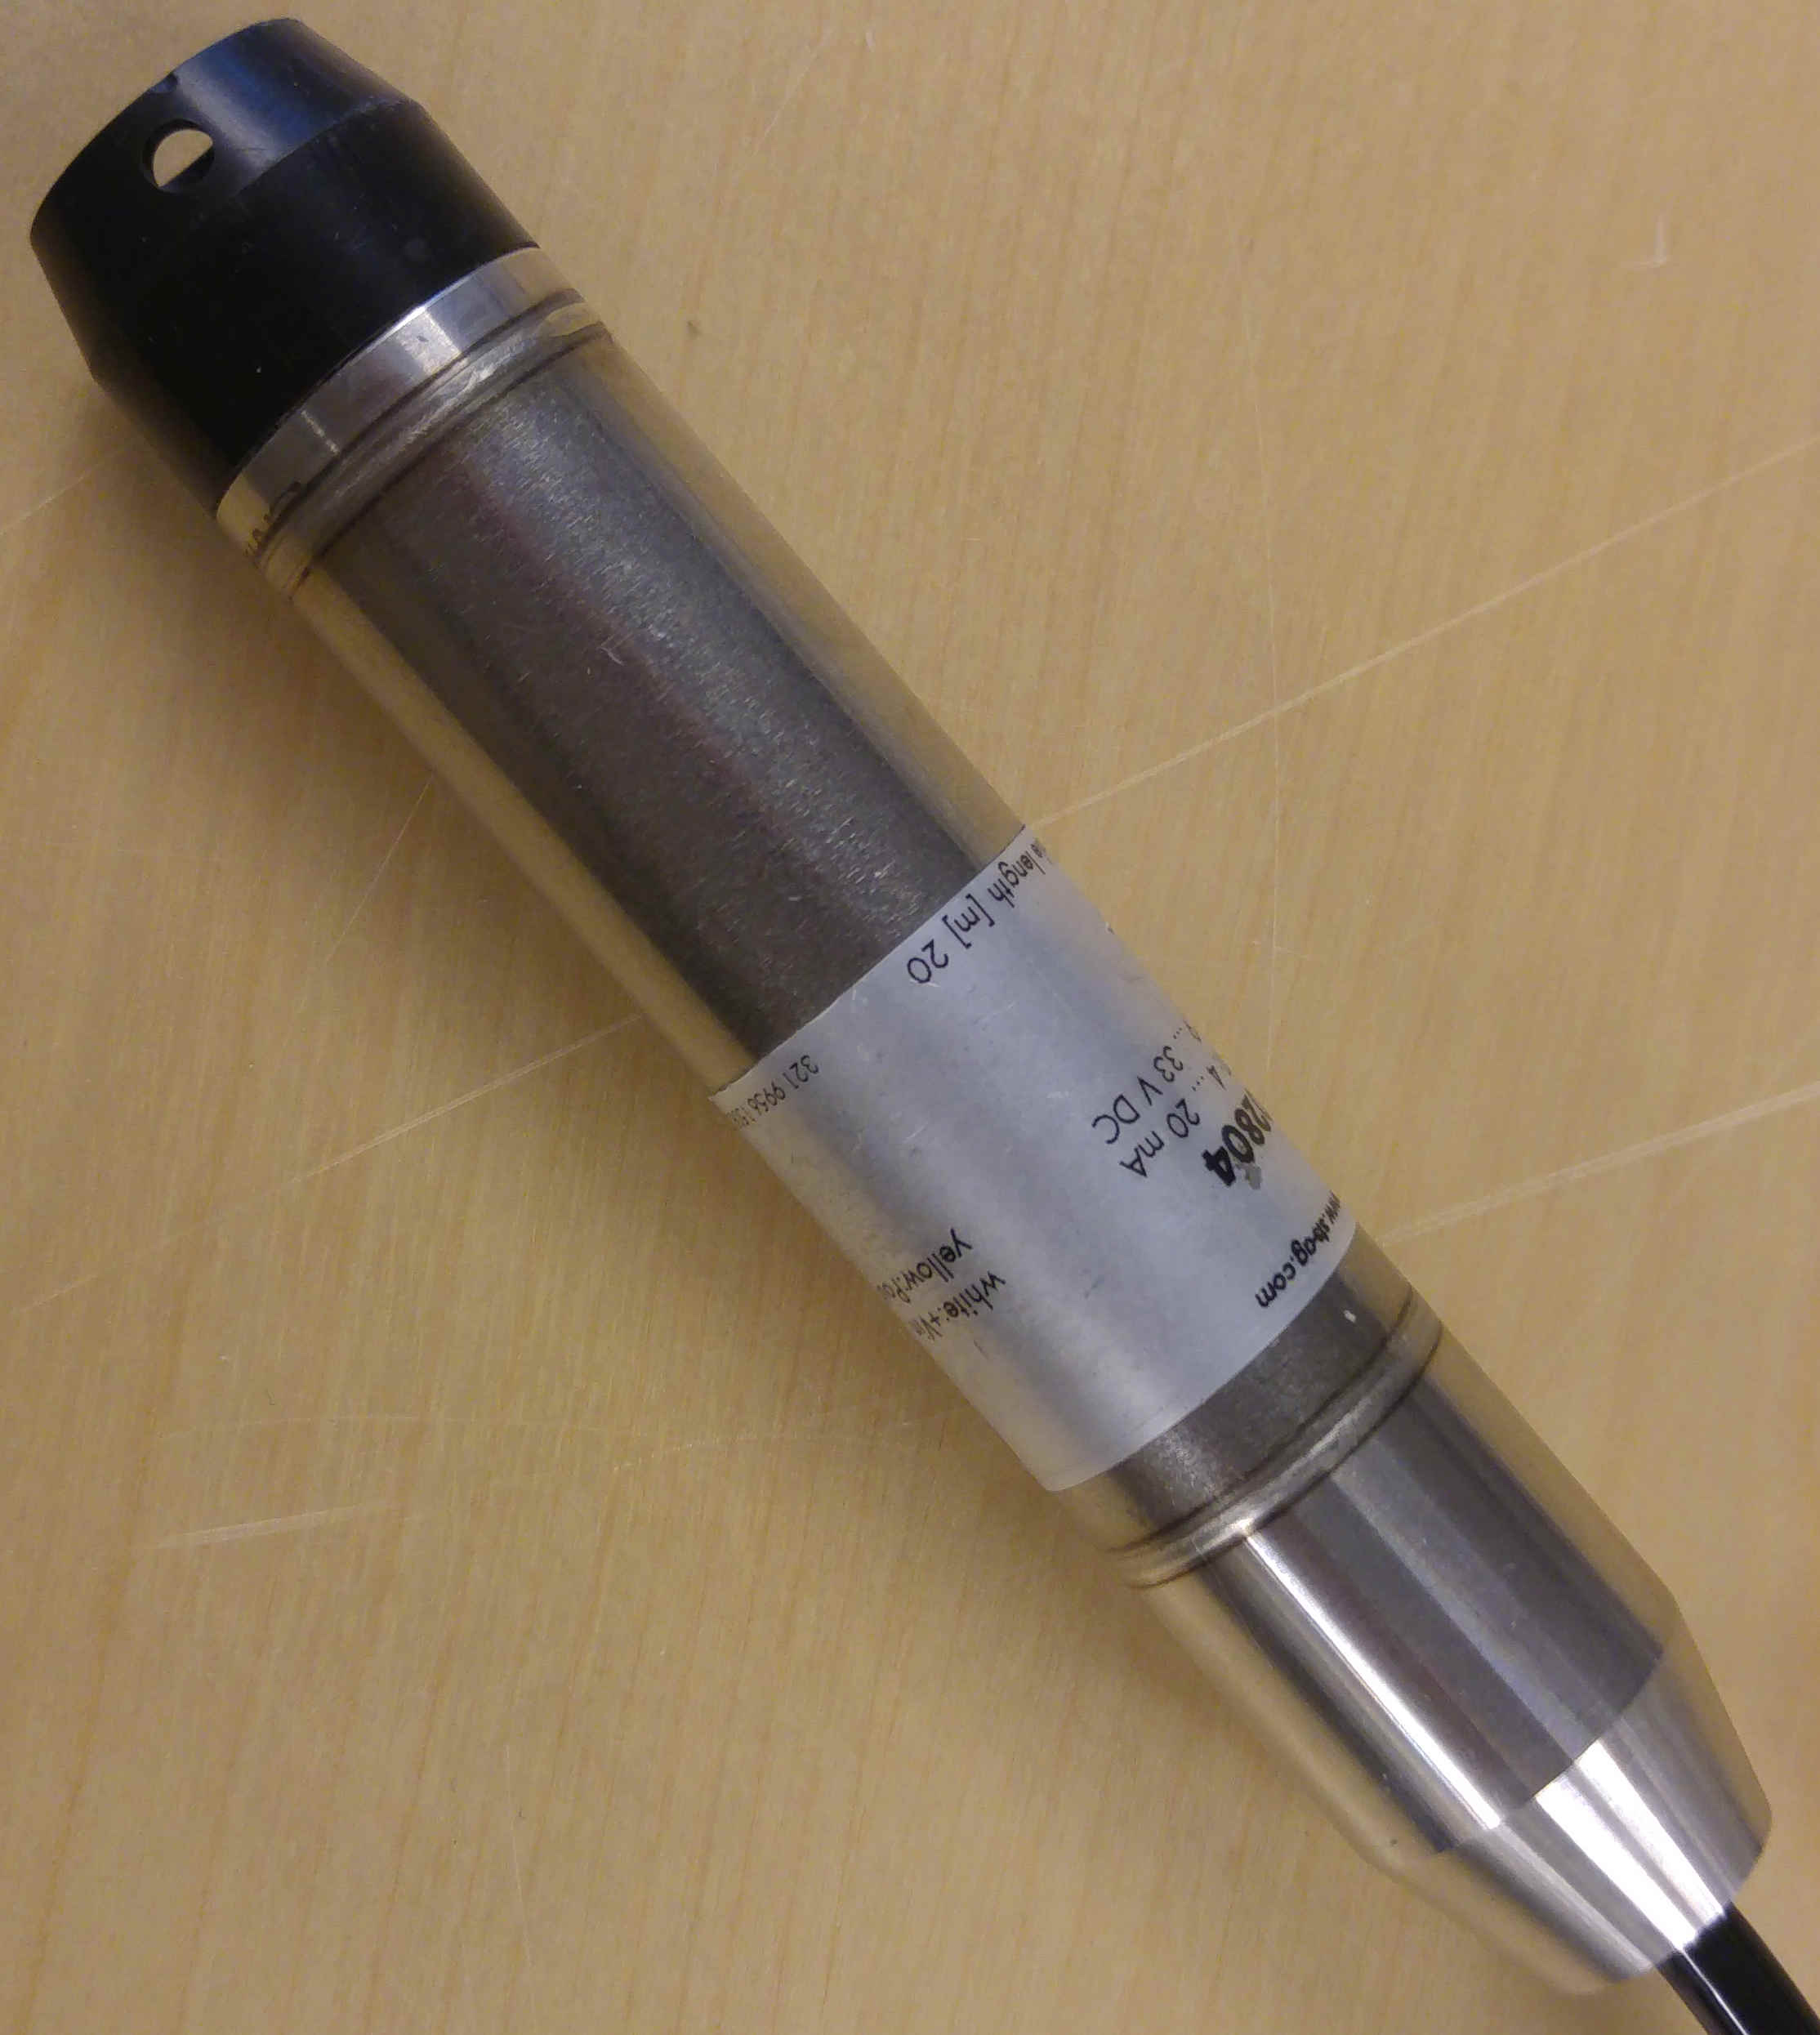
\includegraphics[scale=0.024,angle=0]{pressure_sensor.jpg}
    \caption{Pressure Sensor used to measure the depth of the cable.}
    \label{fig:pressure_sensor}
    \end{minipage}
    \hfill
    \begin{minipage}[b]{0.45\textwidth}
    \centering
    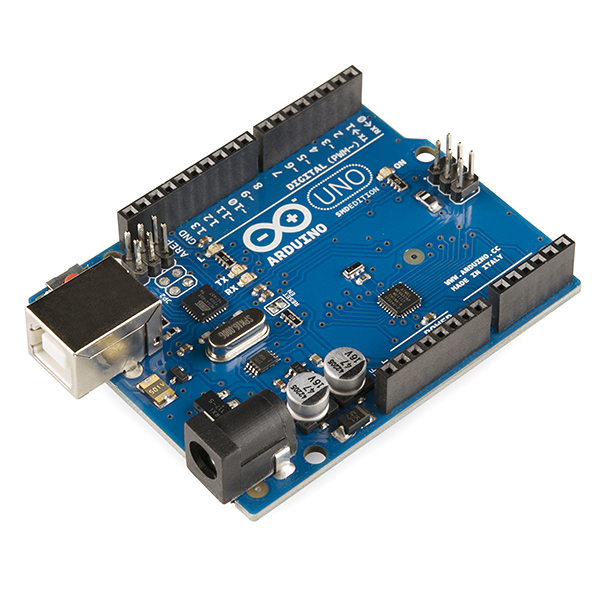
\includegraphics[scale=0.4,angle=0]{arduino_uno.jpg}
    \caption{Arduino Uno as a converter for the pressure sensor.}
    \label{fig:arduino_uno}
    \end{minipage}
\end{figure}

The data was first received be an xBee, a radio transmitter, and logged on a remote computer via Labview, but the data transfer was not reliable enough to get good interpretation of the results. Then the pressure sensor have been incorporated in the database (remote and local) , data is sent live to a web server to be saved and displayed via a 4G modem.

\begin{figure}[H]
\centering
    \begin{minipage}[b]{0.4\textwidth}
    \centering
    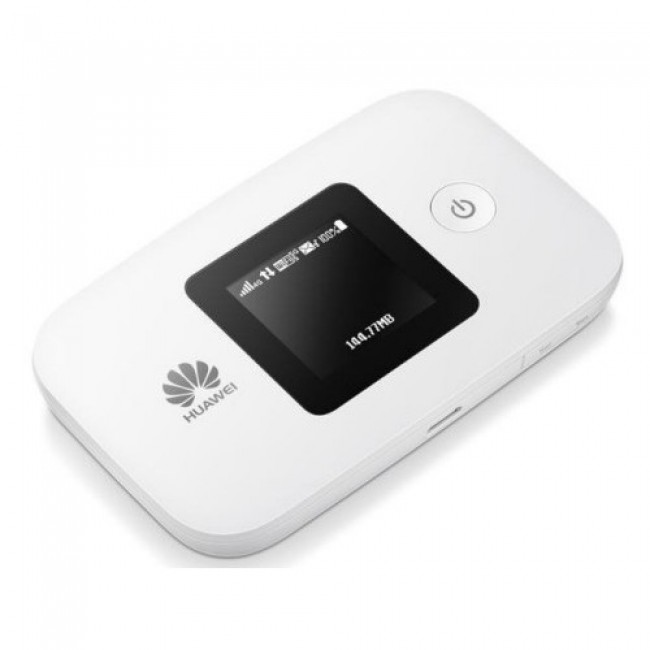
\includegraphics[scale=0.15,angle=0]{4Grouting.jpg}
    \caption{4G Hotspot sending data to the web server.}
    \label{fig:4grouting}
    \end{minipage}
    \hfill
    \begin{minipage}[b]{0.45\textwidth}
    \centering
    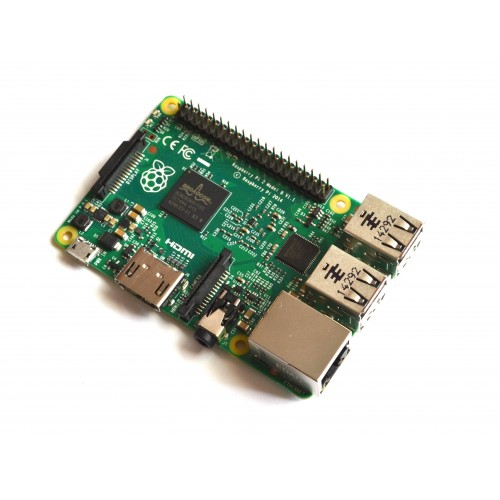
\includegraphics[scale=0.22,angle=0]{raspeberry.jpg}
    \caption{Raspeberry V3 Computing Unit of the sailboat.}
    \label{fig:raspeberry}
    \end{minipage}
\end{figure}

The Raspberry Pi is running Arch Linux and the program controlling the boat is written in C++ (see~\ref{sec:simulator} for more details).

\section{Test process}

First the gathered data will be compared with the old model to see if the new one add any advantage in the design of controller.It is not certain to see a lot a differences between the similarity of each model of the boat to the real test, as said before the model does not take into account the roll of the boat , this can change the expected value of the pressure sensor.

 The goal is to determine is the simulation of the cable is usable and to see if the new model of the boat will be useful in the conception of new controller handling the cable. 
 
 The test procedure is quite simple
 
\begin{itemize}
\item Cable added on the hull of the boat (between 6 and 20 m) with a linear mass of 130 g/m
\item Tapping a pressure sensor on the cable, the length of the cable attached to the pressure sensor is 6 meters
\item Boat has to reach multiple waypoints while measuring the depth of the pressure sensor
\item Boat redo the same path without cable
\end{itemize}

As the pressure sensor cable is smaller than the long one (3 meters in the water), to compare to the simulation, we take the values of the depth of the cable in the simulation at 3 meters length.


\begin{figure}[H]
\centering
    \begin{minipage}[b]{0.4\textwidth}
    \centering
    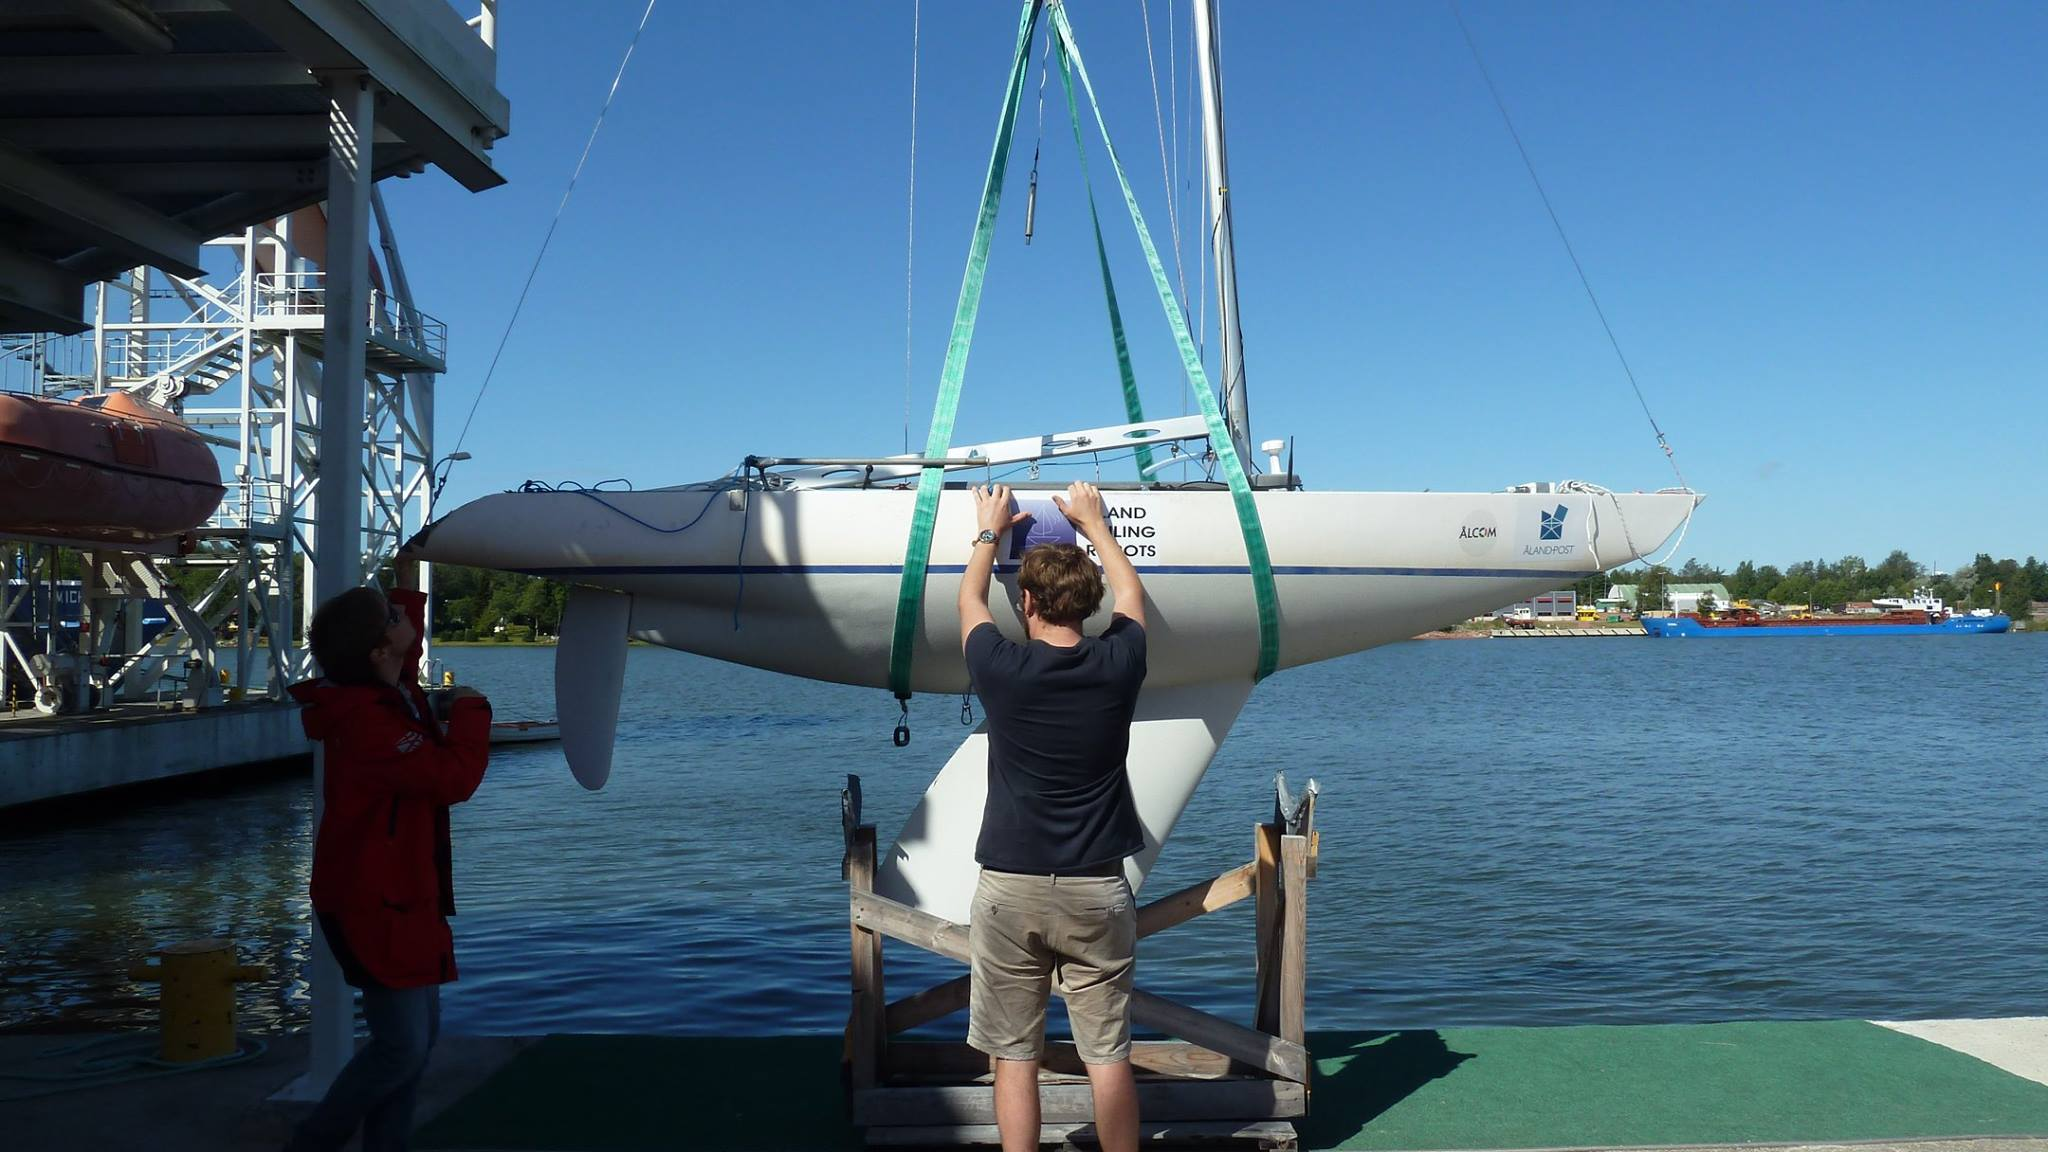
\includegraphics[width=5cm,angle=0]{launching_boat.jpg}
    \caption{Lowering the boat in the water.}
    \label{fig:lowerboat}
    \end{minipage}
    \hfill
    \begin{minipage}[b]{0.45\textwidth}
    \centering
    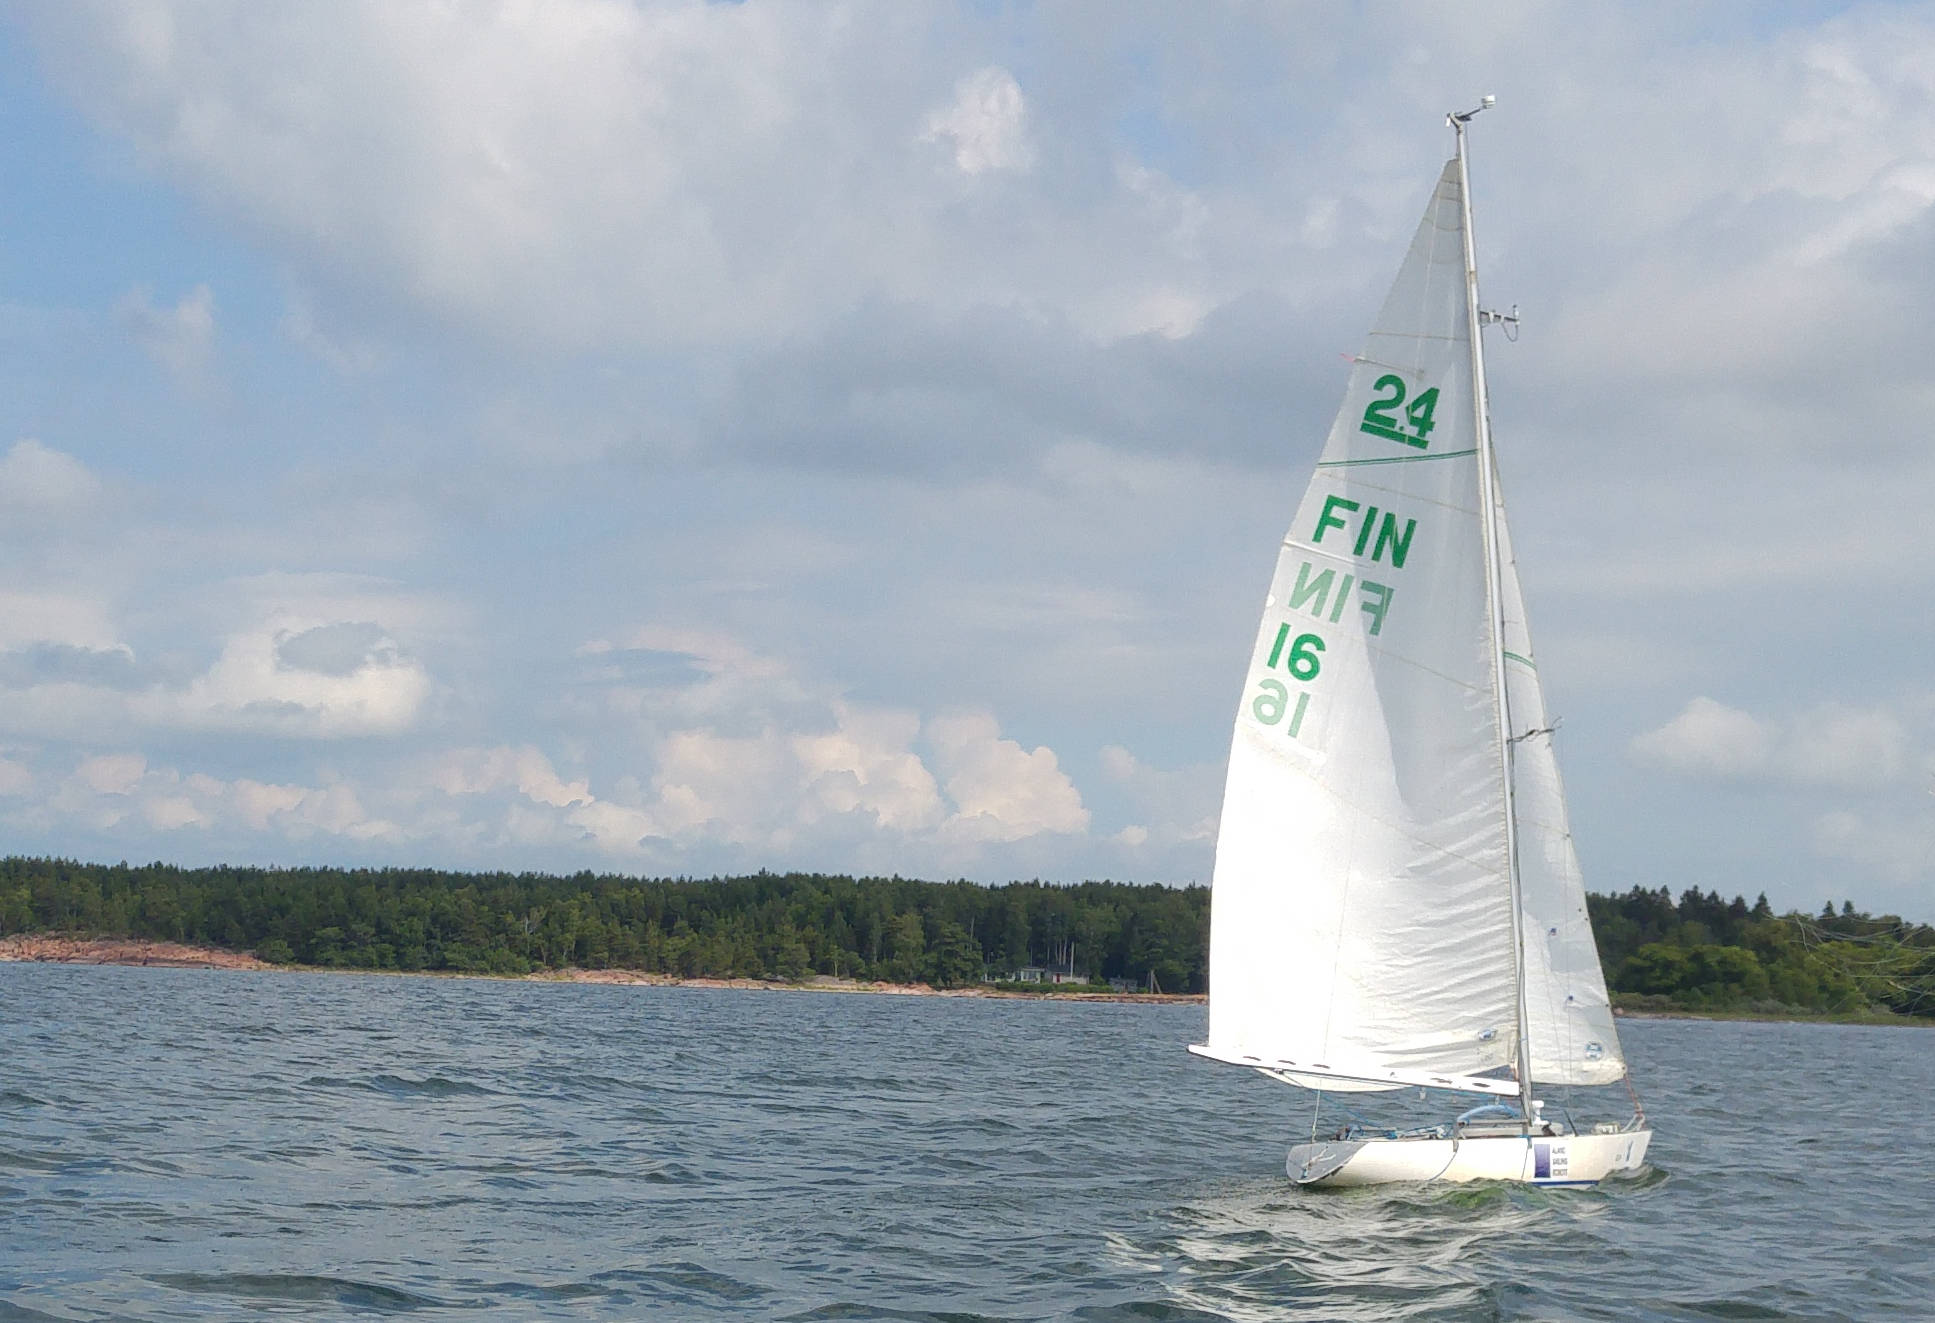
\includegraphics[width=5cm,angle=0]{sailingrobot.jpg}
    \caption{Sailbot sailing during a test.}
    \label{fig:sailbot_test}
    \end{minipage}
\end{figure}

\section{Validation of cable simulation}

First the depth of the pressure sensor will be compared to the depth of the simulation of the cable when taking the speed and position data.

\begin{figure}[H]
\centering
    \begin{minipage}[b]{0.4\textwidth}
    \centering
    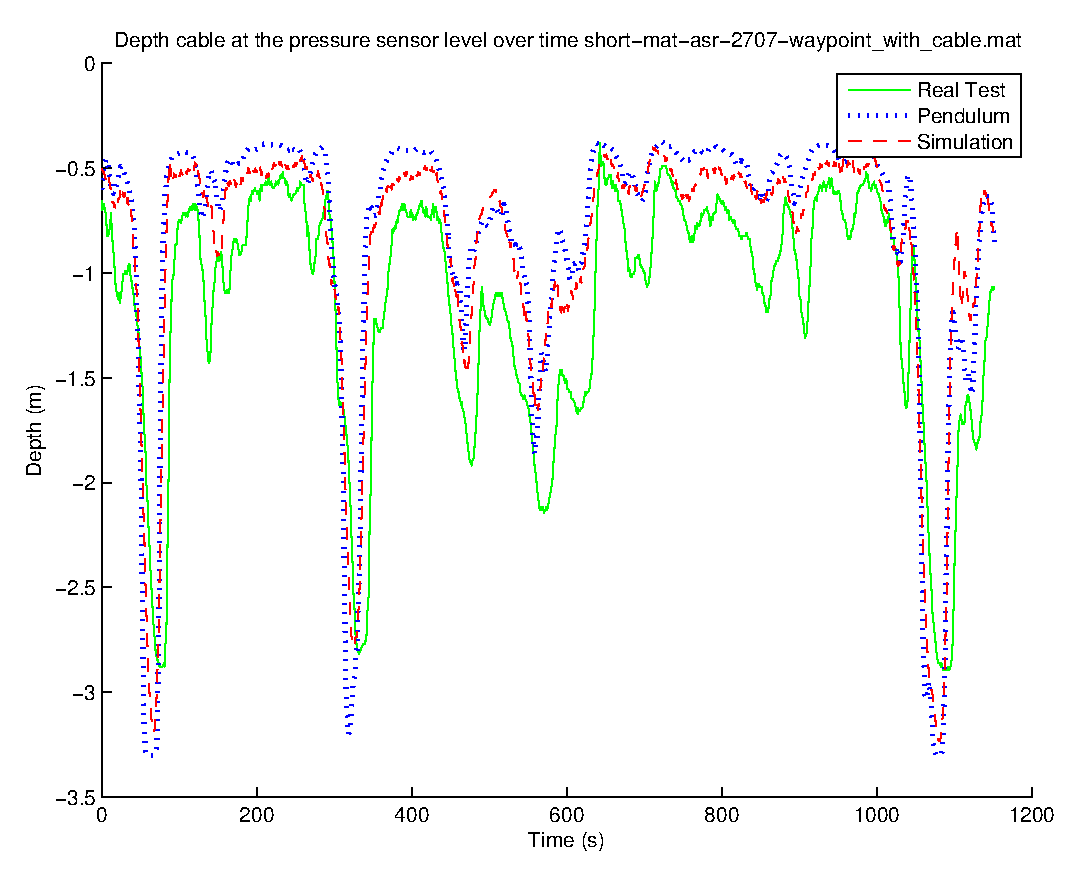
\includegraphics[scale=0.4,angle=0]{depth_time_2707}
    \caption{Comparison between depth of cable at the pressure sensor level in simulation and real test.}
    \label{fig:comp_depth_time_2007}
    \end{minipage}
    \hfill
    \begin{minipage}[b]{0.45\textwidth}
    \centering
    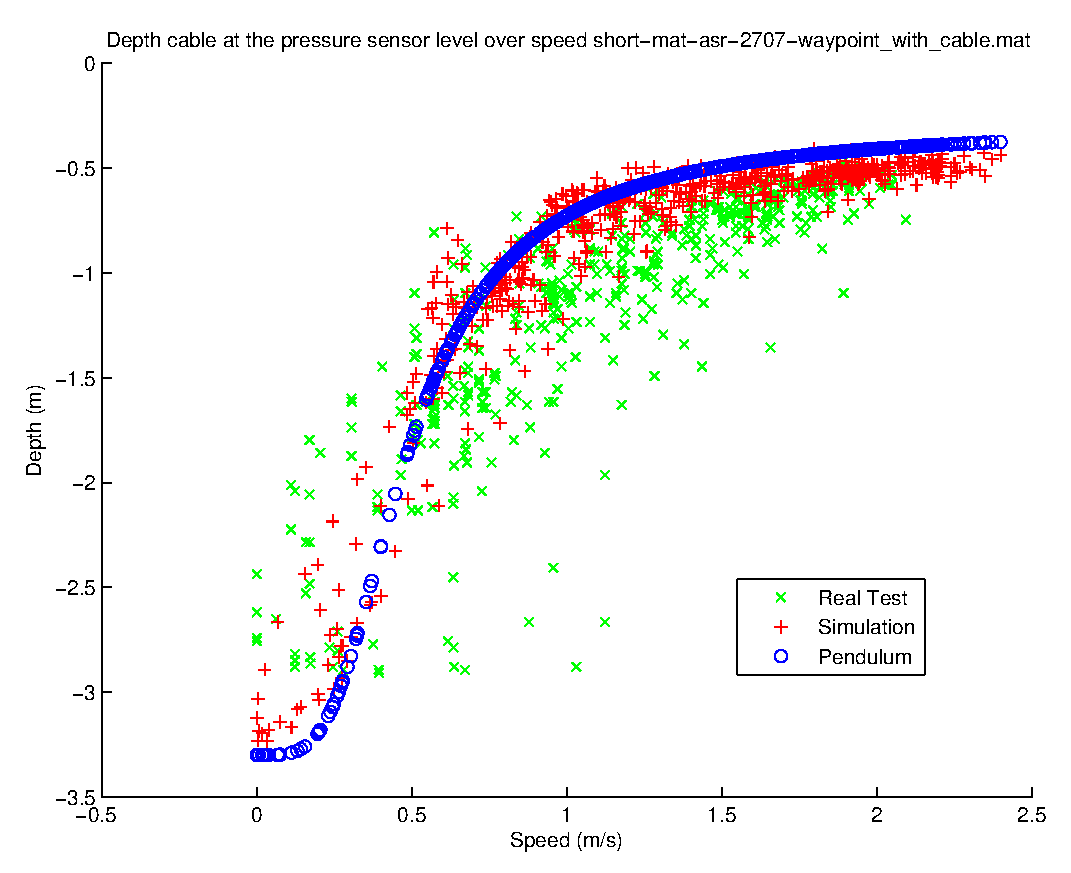
\includegraphics[scale=0.4,angle=0]{depth_speed_2707}
    \caption{Comparison of depth of cable at the pressure sensor level in function of speed between simulation and real test.}
    \label{fig:comp_depth_speed_2007}
    \end{minipage}
\end{figure}

To simulate the run of the boat with the simulation of the cable , the \gls{GPS} position data from the run is taken and filtered, and then feed to the simulator, the cable consider the positions as a fixed point of the cable.

The figure~\ref{fig:comp_depth_time_2007} hold three profile of depth, the real test, the depth computed by simulation and one computed with the formula from~\ref{equ_theta_1}. The first conclusion is that the depth of the cable in the test is similar to the simulation and the profile from the pendulum model too.
 In the same way the profile of depth over speed is also close between test and simulation.
 
 The simulation has an mean offset off 34 cm and the pendulum  43 cm so if we consider the simulation close enough we can consider also the pendulum to be close enough as way to predict the depth of the cable at a certain speed.
 
 \begin{figure}[H]
\centering
    \begin{minipage}[b]{0.4\textwidth}
    \centering
    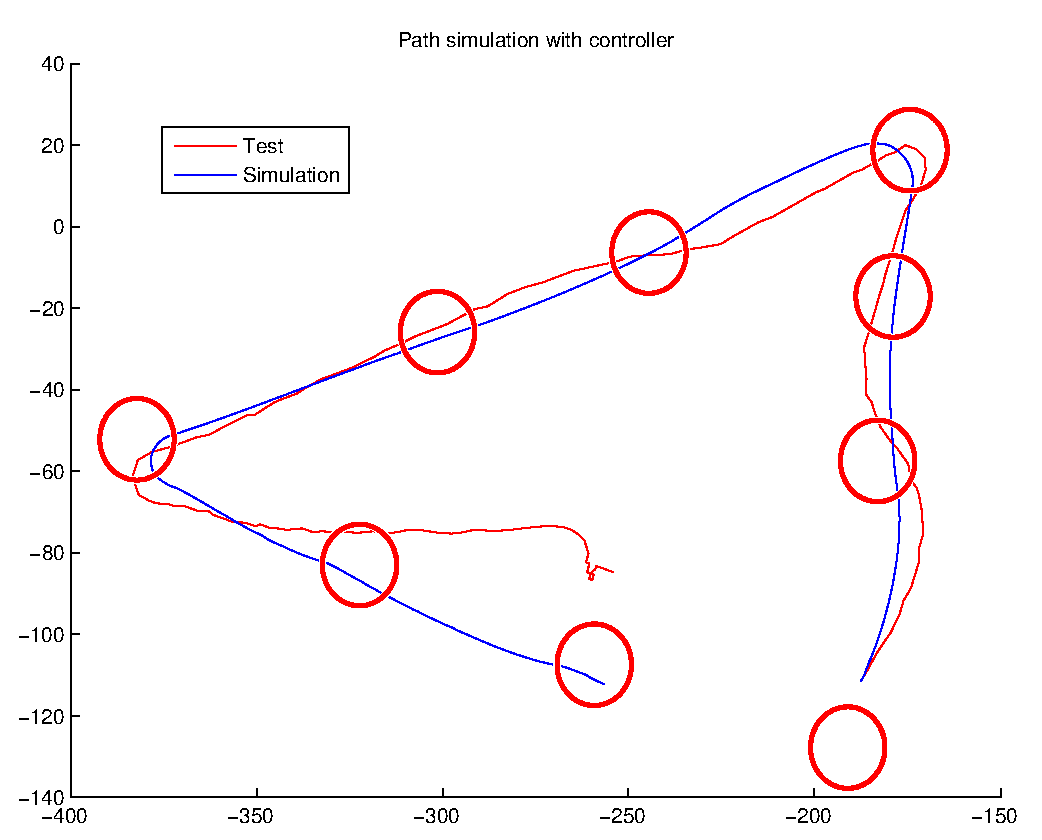
\includegraphics[scale=0.4,angle=0]{simulation_path_controller_with_cable_3006}
    \caption{Comparison of path between simulation and test with cable 416 s.}
    \label{fig:comp_w_cable_3006}
    \end{minipage}
    \hfill
    \begin{minipage}[b]{0.45\textwidth}
    \centering
    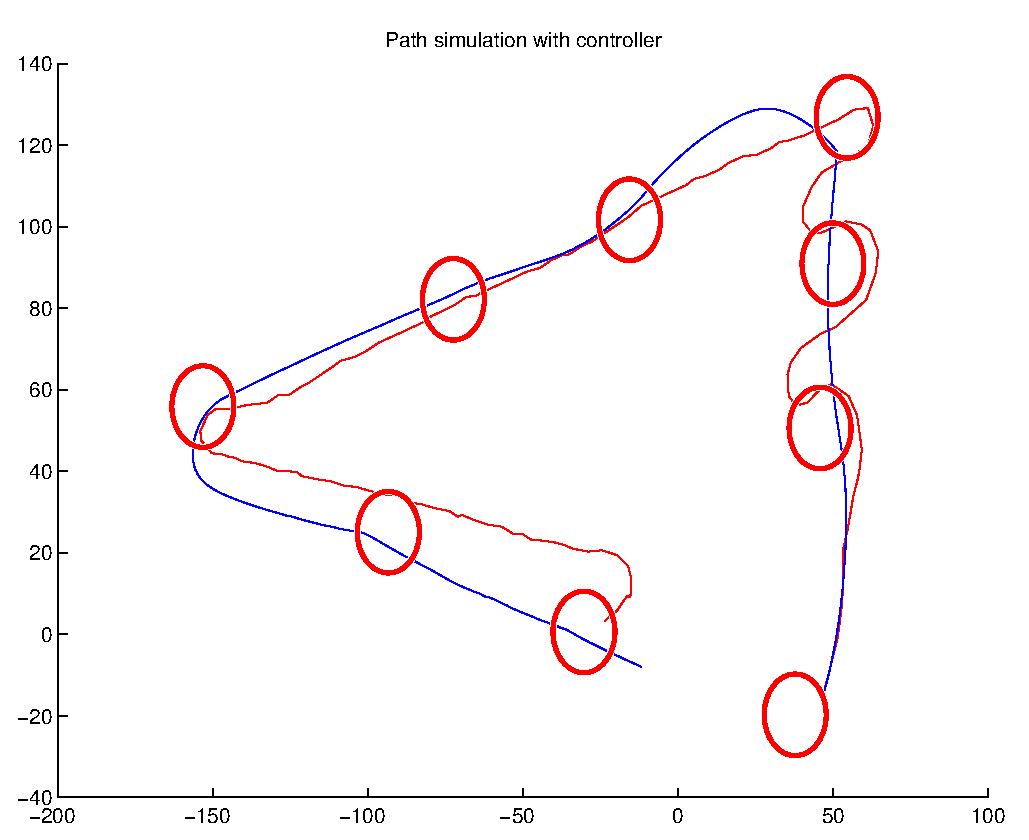
\includegraphics[scale=0.4,angle=0]{simulation_path_controller_without_cable_3006}
    \caption{Comparison of path between simulation and test without cable 430 s.}
    \label{fig:comp_wt_cable_3006}
    \end{minipage}
\end{figure}

In the simulation runs represented in~\ref{fig:comp_w_cable_3006} and~\ref{fig:comp_wt_cable_3006} the simulation follow the same algorithm that the one on the boat.

 \begin{figure}[H]
    \centering
    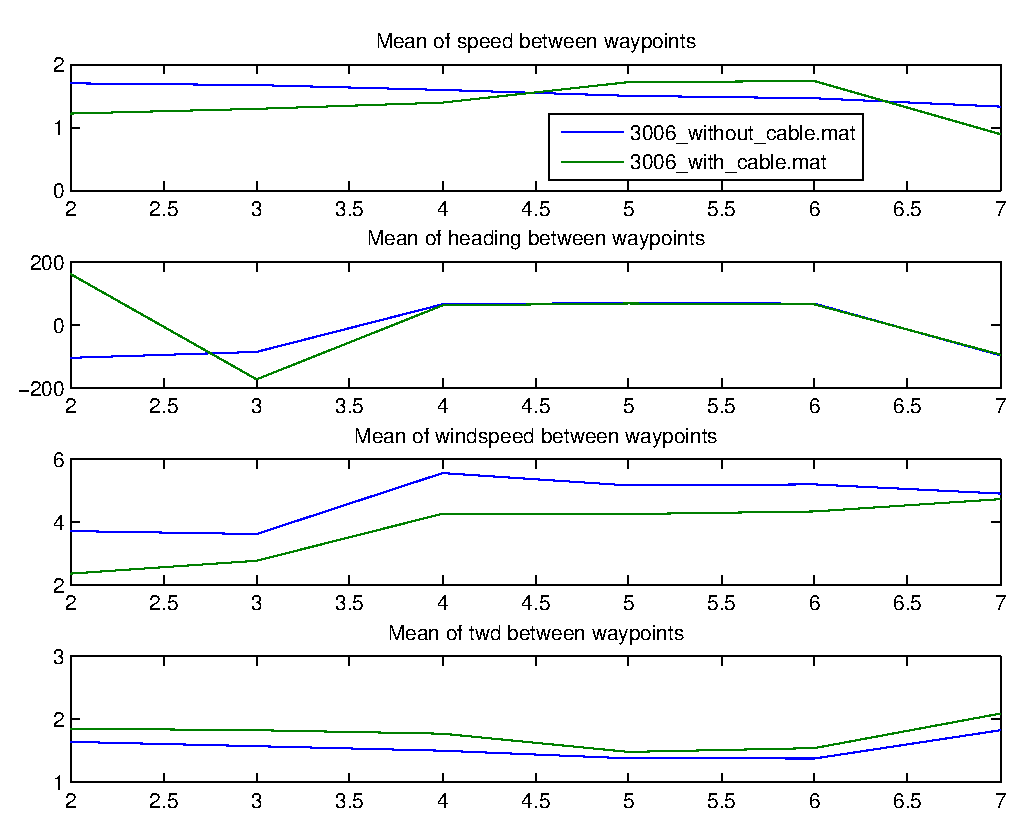
\includegraphics[scale=0.4,angle=0]{comp_run_test_3006}
    \caption{Comparison of some significant values between waypoints for the test.}
    \label{fig:comp_run_306}
\end{figure}

The figure ~\ref{fig:comp_w_cable_3006} compare the speed,heading of the boat and the direction and speed of the wind between a run with the cable and a run without it. The most interesting part is between the waypoints 4 and 7 ( the value at 4 represent the mean value between the waypoints 4 and 5)  because the boat have the same mean heading. At the point 4 the speed of the boat without cable is greater than the speed of the boat without cable however the wind speed is also bigger than the run without cable so we can't conclude that the cable slow down the boat. And at the point 6 the situation is quite odd as the speed of the boat with cable is faster 
even though the wind speed during its run is smaller.

When considering the path of the boat during the simulations runs it is really similar and may change only because of the wind effect.

Considering this it can be supposed that the cable has a little effect on the boat and even in the simulation the differences are not big enough to make the design of a controller require its own model, as long as the cable remains relatively lightweight.
	



 


\section{Proposition of controllers for cable handling}
 The cable for survey operation need to be under a certain depth,from ~\ref{fig:depth_length_speed_pendulum} it can be seen that extend the length of the cable dynamically during the survey will not help because at higher speed the end of the cable reach quickly the surface level. Mass can be added to ensure depth until a certain speed, following ~\ref{fig:depth_mass_speed_pendulum} a cable mass of 9 kilogrammes would ensure a depth of 5 meters for a cable length of 10 meters until 1.5 meters per second.

But to have in general the same depth during a survey the speed of the boat need to be controlled and remain steady. 

One  way to do it be the handling of the sail and using the water resistance to slow down the boat but for this to work would me a perfect sail that wouldn't give any speed when the sail are trimmed in tightly (in ~\ref{fig:drawing_boat_ink} $\delta_s~=~0$).
   Some command can be send to the rudder to make the boat jiggle and lose speed.
 
Some iteration have been made on the design of a controller: 
 
\begin{algorithm}[H]
\caption{Cable Depth sailbot controller using rudder and sail }
\label{alg:breakAlg1}
\begin{algorithmic}[1]
\REQUIRE $depth_{target}$ (< 0), $v_{boat}$\\
   $\delta_s$ : Sail command given by conventional navigation algorithm\\
   $\delta_r$ : Rudder command given by conventional navigation algorithm\\
   $C_D$ : drag coefficient of the cable \\
   $l$ : length of the cable\\
   $\rho$: density of water\\
   $g$ : gravitational constant\\
   $r$ : radius of the cable\\
   $m$ : mass of the cable\\
\STATE $v_{target} \leftarrow \sqrt{\frac{2 g \cdot (m - l \rho \pi r^2)}{C_D l 2 r \rho} \cdot \tan(acos(\frac{-depth_{target}}{l}))}$
\STATE $\Delta_{v} \leftarrow v_{target} - v_{boat}$
\IF{$\Delta_{v} <  0 $}
\STATE $\delta_s \leftarrow 0$
\STATE $\delta_r \leftarrow \delta_r - \textnormal{sign}(\delta_r) \cdot (k_p  \cdot \Delta_v + k_d \cdot \dot{\Delta_v})$
\ENDIF
\end{algorithmic}
\end{algorithm}
 
\begin{figure}[H]
\centering
    \begin{minipage}[b]{0.4\textwidth}
    \centering
    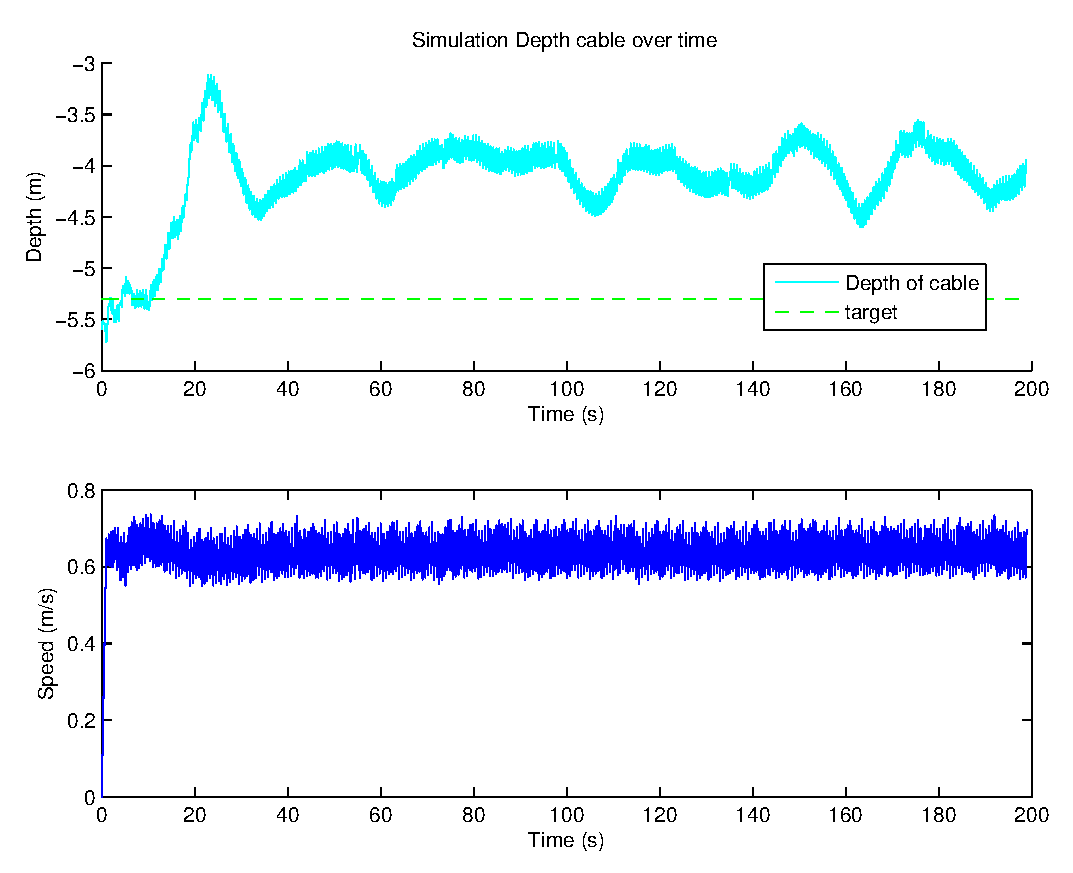
\includegraphics[scale=0.45,angle=0]{depth_controller_speed_rudder_sail_algo1}
    \caption{Depth and speed of the boat under algorithm~\ref{alg:breakAlg1}.}
    \label{fig: algo1Depth}
    \end{minipage}
    \hfill
    \begin{minipage}[b]{0.45\textwidth}
    \centering
    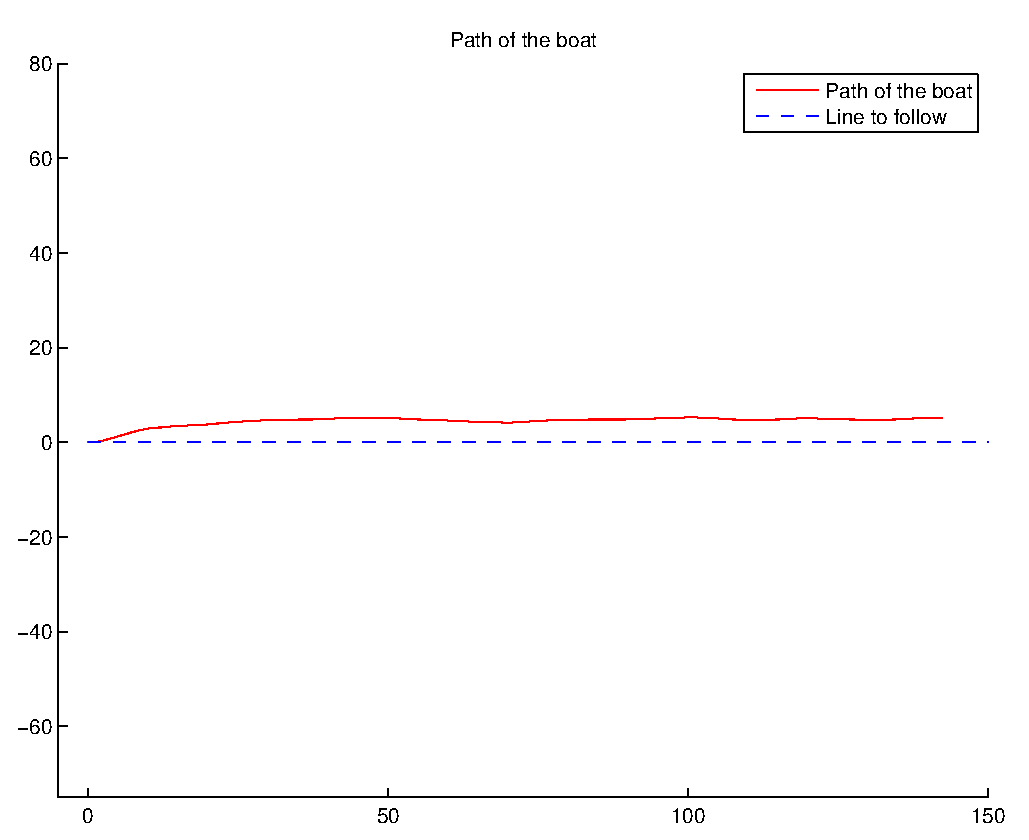
\includegraphics[scale=0.45,angle=0]{depth_controller_path_rudder_sail_algo1}
    \caption{Path of the boat under algorithm~\ref{alg:breakAlg1}.}
    \label{fig:algo1Path}
    \end{minipage}
\end{figure}
 
Using the rudder to slow down the boat is does not seem to be an efficient idea as seen in~\ref{fig:algo1Path} the boat is not following the line exactly around 5 meters off the line (initial condition is the boat is directly on the right path and downwind. The speed is also not steady and fluctuate a lot during the run.

 Then the test can be done with only controlling the sail for managing the speed here a PID controller:


\begin{algorithm}[H]
\caption{PID Speed sailbot controller using sail only}
\label{alg:breakAlg2}
\begin{algorithmic}[1]
\REQUIRE $v_{target}$, $v_{boat}$\\
   $\delta_s$ : Sail command given by conventional navigation algorithm\\
   $\delta_r$ : Rudder command given by conventional navigation algorithm\\
   $K_D$ : derivative coefficient for the PID controller $ K_D < 0$\\
   $K_I$ : integral coefficient for the PID controller $ K_I < 0$\\
\STATE $\Delta_{v} \leftarrow v_{target} - v_{boat}$
\IF{$\Delta_{v} \leq  0 $}
\STATE $\delta_s \leftarrow 0$
\ELSE
\IF{$v_{boat} > 0$}
\STATE $\delta_s \leftarrow \delta_s \cdot (\frac{\Delta_v}{v_{target}} + K_D \cdot \dot{\Delta}_v + K_I \cdot \displaystyle \int \Delta_v )$
\ENDIF
\ENDIF
\end{algorithmic}
\end{algorithm}

\begin{figure}[H]
\centering
    \begin{minipage}[b]{0.4\textwidth}
    \centering
    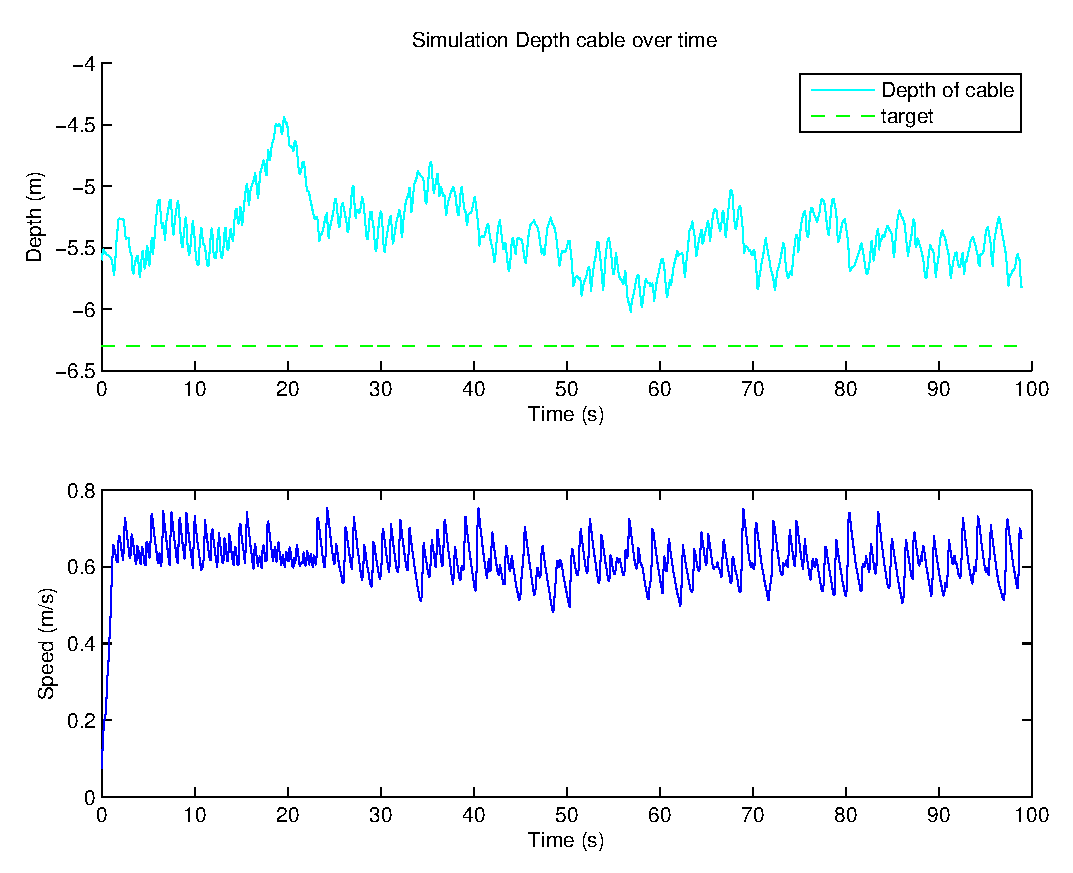
\includegraphics[scale=0.45,angle=0]{depth_controller_speed_rudder_sail_algo2}
    \caption{Depth and speed of the boat under algorithm~\ref{alg:breakAlg1}.}
    \label{fig: algo2Depth}
    \end{minipage}
    \hfill
    \begin{minipage}[b]{0.45\textwidth}
    \centering
    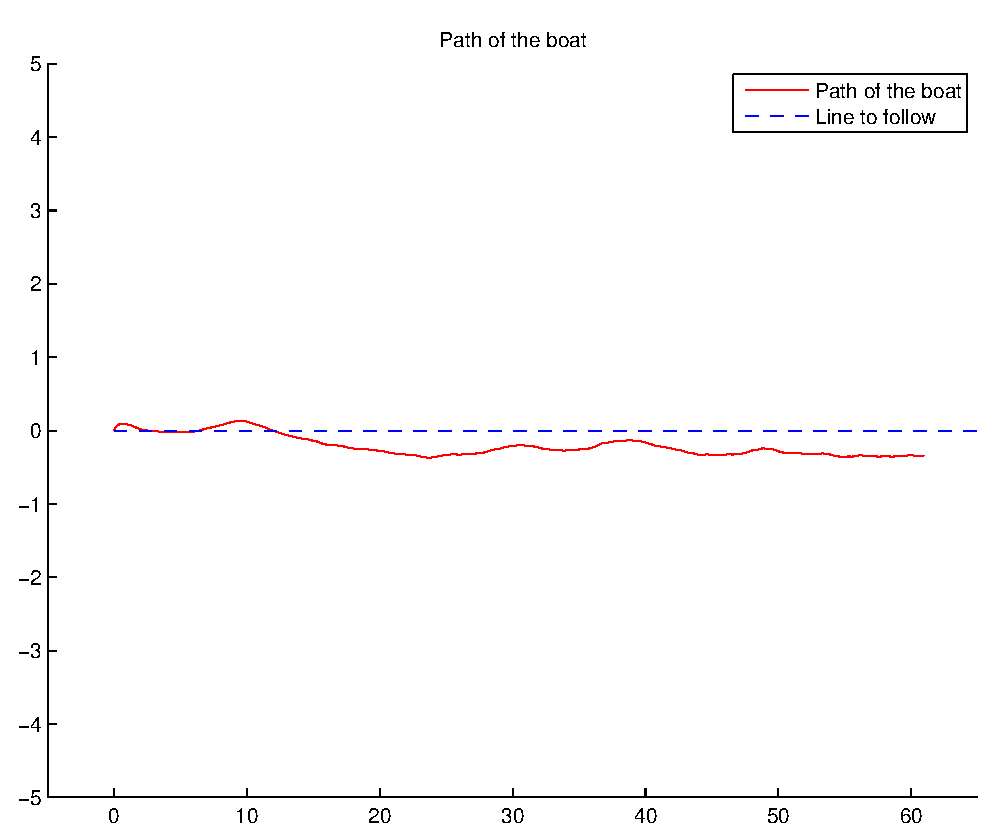
\includegraphics[scale=0.45,angle=0]{depth_controller_path_rudder_sail_algo2}
    \caption{Path of the boat under algorithm~\ref{alg:breakAlg1}.}
    \label{fig:algo2Path}
    \end{minipage}
\end{figure}

The PID controller does not completely solve the problem of the the algorithm~\ref{alg:breakAlg1}, the error of the path taken by the boat is reduce boat  it still seems to have an offset (~\ref{fig:algo2Path}). This also induce oscillation that may not be good for the measurement on a survey.

The following algorithm is a modified version of a proportional controller as there is no derivative or integral term but the output is not, see~\ref{fig:responAlgo3} for the profile of the sail command depending on the speed error.

\begin{figure}[H]
\centering
    \begin{minipage}[b]{0.4\textwidth}
    \begin{algorithm}[H]
\caption{Speed sailbot controller using sail only}
\label{alg:breakAlg3}
\begin{algorithmic}[1]
\REQUIRE $v_{target}$, $v_{boat}$\\
   $\delta_s$ : Sail command\\
   $\delta_r$ : Rudder command\\
   $k$ : coefficient $(0< k <1)$\\
\STATE $\Delta_{v} \leftarrow v_{target} - v_{boat}$
\IF{$\Delta_{v} \leq  0 $}
\STATE $\delta_s \leftarrow 0$
\ELSE
\STATE $\delta_s \leftarrow \delta_s \cdot  \exp(-k \cdot (\frac{v_{target}}{\Delta_v}-1)) $
\ENDIF
\end{algorithmic}
\end{algorithm}
    \end{minipage}
    \hfill
    \begin{minipage}[b]{0.45\textwidth}
    \centering
    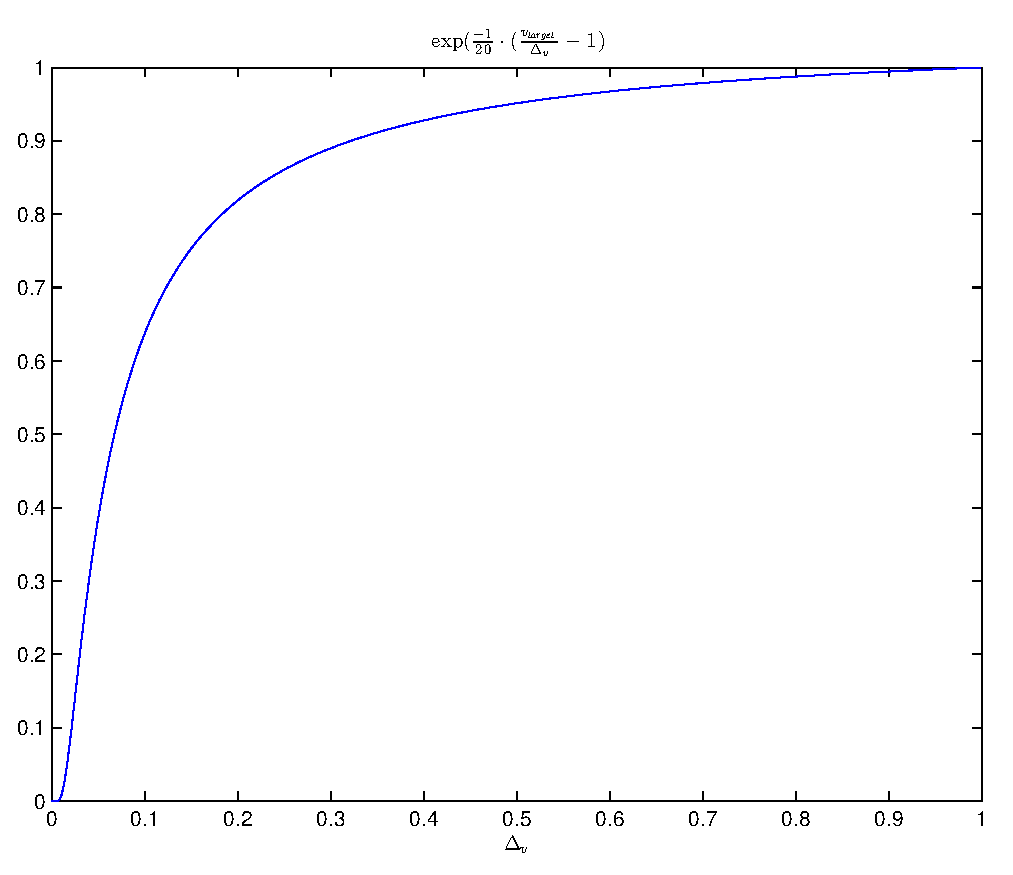
\includegraphics[scale=0.45,angle=0]{response_algo3}
    \caption{Path of the boat under algorithm}
    \label{fig:responAlgo3}
    \end{minipage}
\end{figure}




\begin{figure}[H]
\centering
    \begin{minipage}[b]{0.4\textwidth}
    \centering
    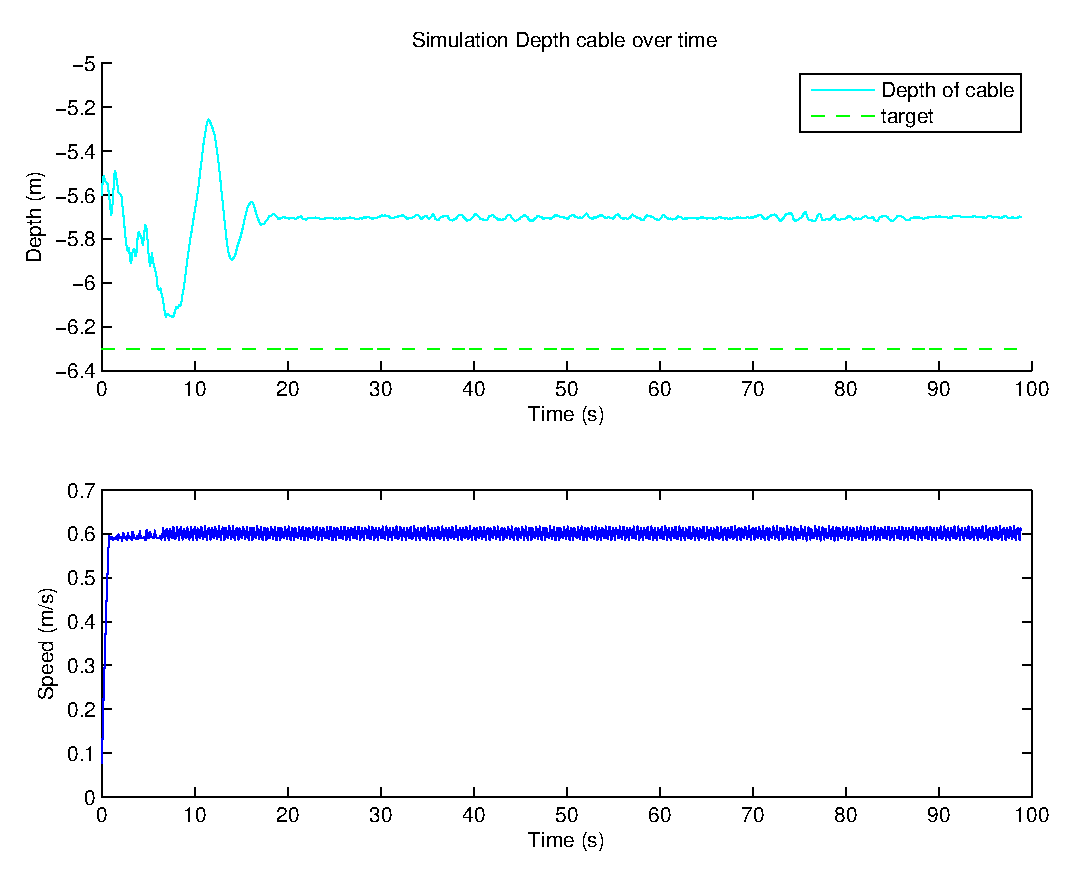
\includegraphics[scale=0.45,angle=0]{depth_controller_speed_rudder_sail_algo3}
    \caption{Depth and speed of the boat under algorithm~\ref{alg:breakAlg1}.}
    \label{fig: algo3Depth}
    \end{minipage}
    \hfill
    \begin{minipage}[b]{0.45\textwidth}
    \centering
    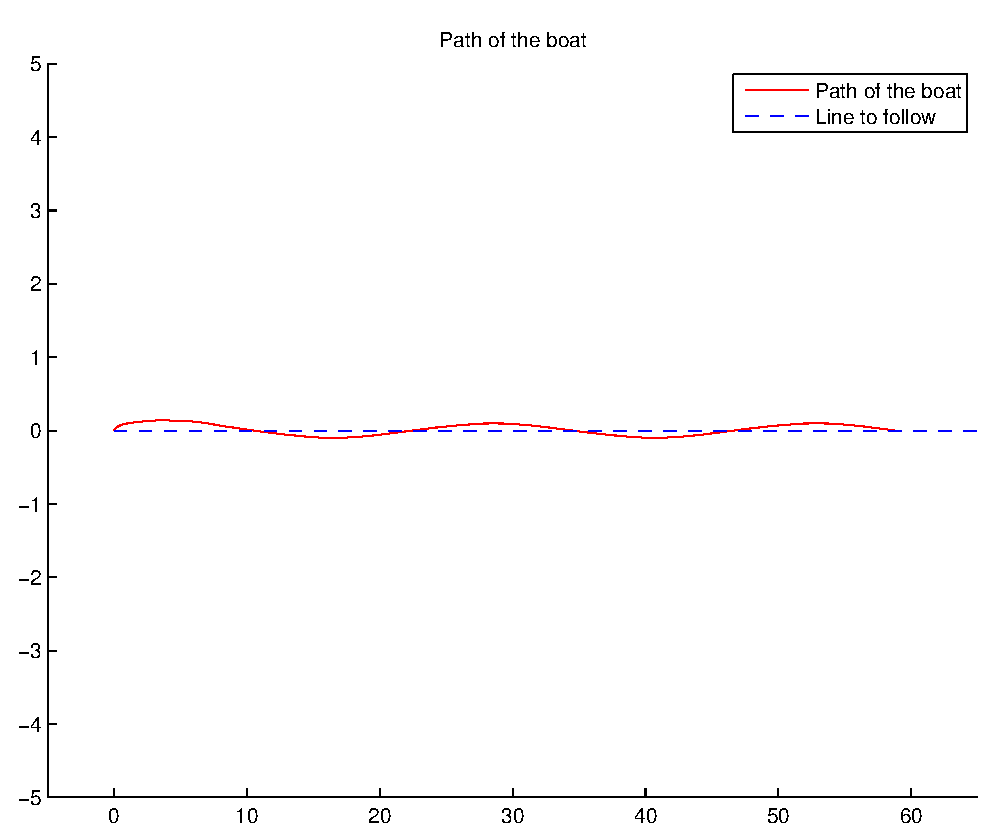
\includegraphics[scale=0.45,angle=0]{depth_controller_path_rudder_sail_algo3}
    \caption{Path of the boat under algorithm~\ref{alg:breakAlg1}.}
    \label{fig:algo3Path}
    \end{minipage}
\end{figure}

The algorithm~\ref{alg:breakAlg3} seems to be working on simulation, but suppose that when $\delta_s = 0$ the wind does not have any effect on the boat. But in general the main sail in itself is not rigid therefore the wind will still have an effect on the boat. They also have a front sail which is not controlled and will make the boat go forward. If these two non controllable are more powerful than the friction of the water then the boat will not be able to slow down to the right speed with only the control of the sail.

A solution to resolve this problem would to put weight on the cable so that the minimal speed increases (see~\ref{fig:depth_length_speed_pendulum}), adding length to the cable would not help on normal speed (1-4 m/s).


An another solution would be to add to the boat a device that would counter the effect of the front sail and the remaining of the main sail. Something simple as board placed to slow down , the surface of this board could be computed to match the push created by the sails.
 
A more advance solution would be to have controllable flap as some foiling boat could have but without  making the boat go up or down.The effect need to be symmetric to the horizontal line :

\begin{figure}[H]
\centering
\psscalebox{0.5 0.5} % Change this value to rescale the drawing.
{
% \usepackage[usenames,dvipsnames]{pstricks}
% \usepackage{epsfig}
% \usepackage{pst-grad} % For gradients
% \usepackage{pst-plot} % For axes
% \usepackage[space]{grffile} % For spaces in paths
% \usepackage{etoolbox} % For spaces in paths
% \makeatletter % For spaces in paths
% \patchcmd\Gread@eps{\@inputcheck#1 }{\@inputcheck"#1"\relax}{}{}
% \makeatother
% % User Packages:
% \usepackage{amsmath}
% \usepackage{amsfonts}
% \usepackage{amssymb}
% \usepackage{algorithm}
% \usepackage{algorithmic}
% 
\psscalebox{1.0 1.0} % Change this value to rescale the drawing.
{
\begin{pspicture}(0,-2.594394)(13.178725,2.594394)
\psline[linecolor=black, linewidth=0.04](0.01,-1.21312)(13.178696,-1.2357286)
\psline[linecolor=black, linewidth=0.04](6.599347,2.5943327)(6.5893474,-1.2556674)
\psframe[linecolor=black, linewidth=0.04, dimen=outer](3.23,0.16560608)(0.0,-1.2043939)
\psframe[linecolor=black, linewidth=0.04, dimen=outer](6.42,-1.214394)(3.19,-2.584394)
\psframe[linecolor=black, linewidth=0.04, dimen=outer](9.97,-1.224394)(6.74,-2.594394)
\psframe[linecolor=black, linewidth=0.04, dimen=outer](13.16,0.12560607)(9.93,-1.244394)
\rput[bl](4.49,1.785606){{\Large Flap} }
\psline[linecolor=black, linewidth=0.02, arrowsize=0.05291667cm 2.0,arrowlength=1.4,arrowinset=0.0]{->}(4.4,1.6856061)(2.5,0.38560608)
\psline[linecolor=black, linewidth=0.02, arrowsize=0.05291667cm 2.0,arrowlength=1.4,arrowinset=0.0]{->}(4.84,1.4756061)(4.66,-0.9243939)
\psline[linecolor=black, linewidth=0.02, arrowsize=0.05291667cm 2.0,arrowlength=1.4,arrowinset=0.0]{->}(5.68,1.6156061)(8.03,-1.0043939)
\psline[linecolor=black, linewidth=0.02, arrowsize=0.05291667cm 2.0,arrowlength=1.4,arrowinset=0.0]{->}(6.01,1.9256061)(9.61,-0.20439392)
\end{pspicture}
}


}
\caption*{Example of manipulable flap to put under the boat.}
\label{fig:model_boat_}
\end{figure}




%\addcontentsline{toc}{part}{Conclusion}
%----------------------------------------------------------------------------------------
%%\appendix
%\chapter{Appendix 1}
\section*{Acknowledgement}

This research has been funded by the Regional European development Fund
%----------------------------------------------------------------------------------------
%	BIBLIOGRAPHIE
%----------------------------------------------------------------------------------------
%\addcontentsline{toc}{part}{Bibliography}
%\bibliographystyle{apalike-fr}
\bibliographystyle{IEEEtran}
\bibliography{bibliographie}
\addcontentsline{toc}{part}{Bibliography}
\nocite{*}


%----------------------------------------------------------------------------------------

\end{document}